\documentclass[11pt]{beamer}
\usetheme{Marcantoni}

\usepackage[utf8]{inputenc}
\usepackage[english]{babel}
\usepackage{amsmath}
\usepackage{amsfonts}
\usepackage{amssymb}
\usepackage{graphicx}
\usepackage{hyperref}
\usepackage{csquotes}
\usepackage{biblatex}
\usepackage{tikz}

\addbibresource{bibliography.bib}

\newcommand{\versionmajor}{0}
\newcommand{\versionminor}{1}
\newcommand{\versionpatch}{0}
\newcommand{\version}{\versionmajor.\versionminor.\versionpatch}

\newcommand{\disi}{Computer Science and Engineering Department (DISI)}
\author[A. Marcantoni]{Alessandro Marcantoni}
\title[Visual Programming Paradigm for Organizations in MAS]{Visual Programming Paradigm for Organizations in Multi-Agent Systems}
\subtitle{\vspace{0.2cm}\emph{Thesis in} \textbf{Pervasive Computing}}
\institute[]{\disi\\Alma Mater Studiorum - Universit\`{a} di Bologna} 
\date[\today]{Academic Year 2021/2022}

\newcommand{\moise}{$\mathcal{M}\text{\footnotesize{OISE}}$}

\begin{document}

\begin{frame}
    \titlepage
\end{frame}

% \begin{frame}[t,allowframebreaks]{Outline}
%     \tableofcontents
% \end{frame}

\begin{frame}{Introduction}
    Context:
    \begin{itemize}
        \item Collaboration with the Interaction- and Communication-
        based Systems research group at the University of St.\ Gallen
        \begin{itemize}
            \item \emph{IntellIoT} European project
            \item Multi-Agent Systems (MAS) applied to IoT
        \end{itemize}
    \end{itemize}
    \vspace{1cm}
    Result:
    \begin{itemize}
        \item Development of a tool that domain experts can use to
        intuitively design MAS organizations
    \end{itemize}
\end{frame}

\section{Context}
\subsection{The \textit{IntellIoT} Project}

\begin{frame}{The \textit{IntellIoT} Project}
    \begin{block}{The Next Generation IoT}
        IntellIoT is a Pan-European project focused on developing integrated, distributed, human-centered, and trustworthy IoT frameworks
    \end{block}

    \begin{columns}
        \begin{column}{0.45\textwidth}
            \begin{itemize}
                \item One of the project's missions is to enable \textbf{domain experts} to define complex systems intuitively
            \end{itemize}
        \end{column}
        \begin{column}{0.55\textwidth}
            \begin{figure}
                \centering
                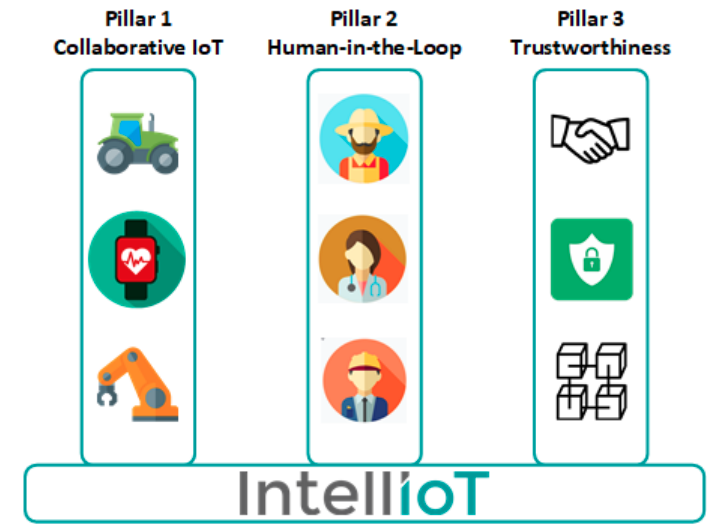
\includegraphics[width=0.8\textwidth]{images/intelliot-pillars.png}
            \end{figure}
        \end{column}
    \end{columns}
\end{frame}
\section{Background \& Motivations}

\subsection{Multi-Agent Systems}
\begin{frame}{Multi-Agent Systems}
    \begin{columns}
        \begin{column}{0.45\textwidth}
            \begin{itemize}
                \item The model chosen by \emph{IntellIoT} for designing and implementing complex IoT systems is represented by \textbf{Multi-Agent Systems} (MAS)
            \end{itemize}
        \end{column}
        \begin{column}{0.55\textwidth}
            \begin{figure}
                \centering
                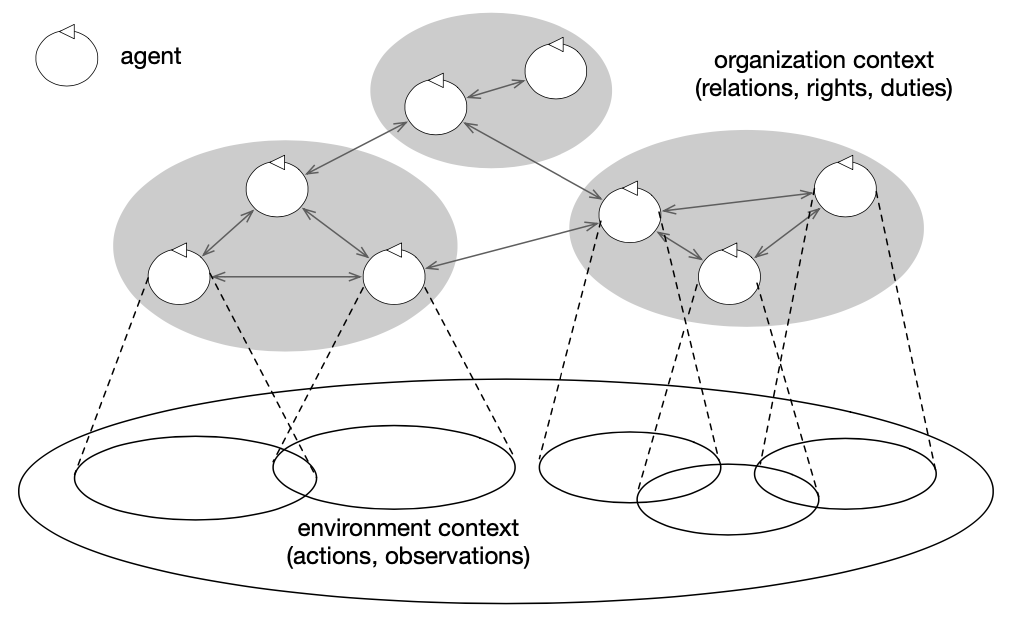
\includegraphics[width=0.8\textwidth]{images/multi-agent-systems.png}
            \end{figure}
        \end{column}
    \end{columns}

    \vspace{0.5cm}

    \begin{block}{Multi-Agent System}
        A MAS consists of multiple decision-making agents interacting in a shared environment to achieve common or conflicting goals~\cite{turing}
    \end{block}
\end{frame}

\begin{frame}{Multi-Agent Oriented Programming}
    \begin{block}{Multi-Agent Oriented Programming}
        MAOP is an approach to programming MAS that promotes the use of three first-class programming abstractions: the \textbf{agent} dimension, the \textbf{environment} dimension, and the \textbf{organization} dimension~\cite{boissier2020multi}
    \end{block}

    \begin{columns}
        \begin{column}{0.4\textwidth}
            \begin{itemize}
                \item JaCaMo is the open-source technology adopted to support the integration of tools and languages for programming the three dimensions of MAOP~\cite{boissier2020multi}
            \end{itemize}
        \end{column}
        \begin{column}{0.6\textwidth}
            \begin{figure}
                \centering
                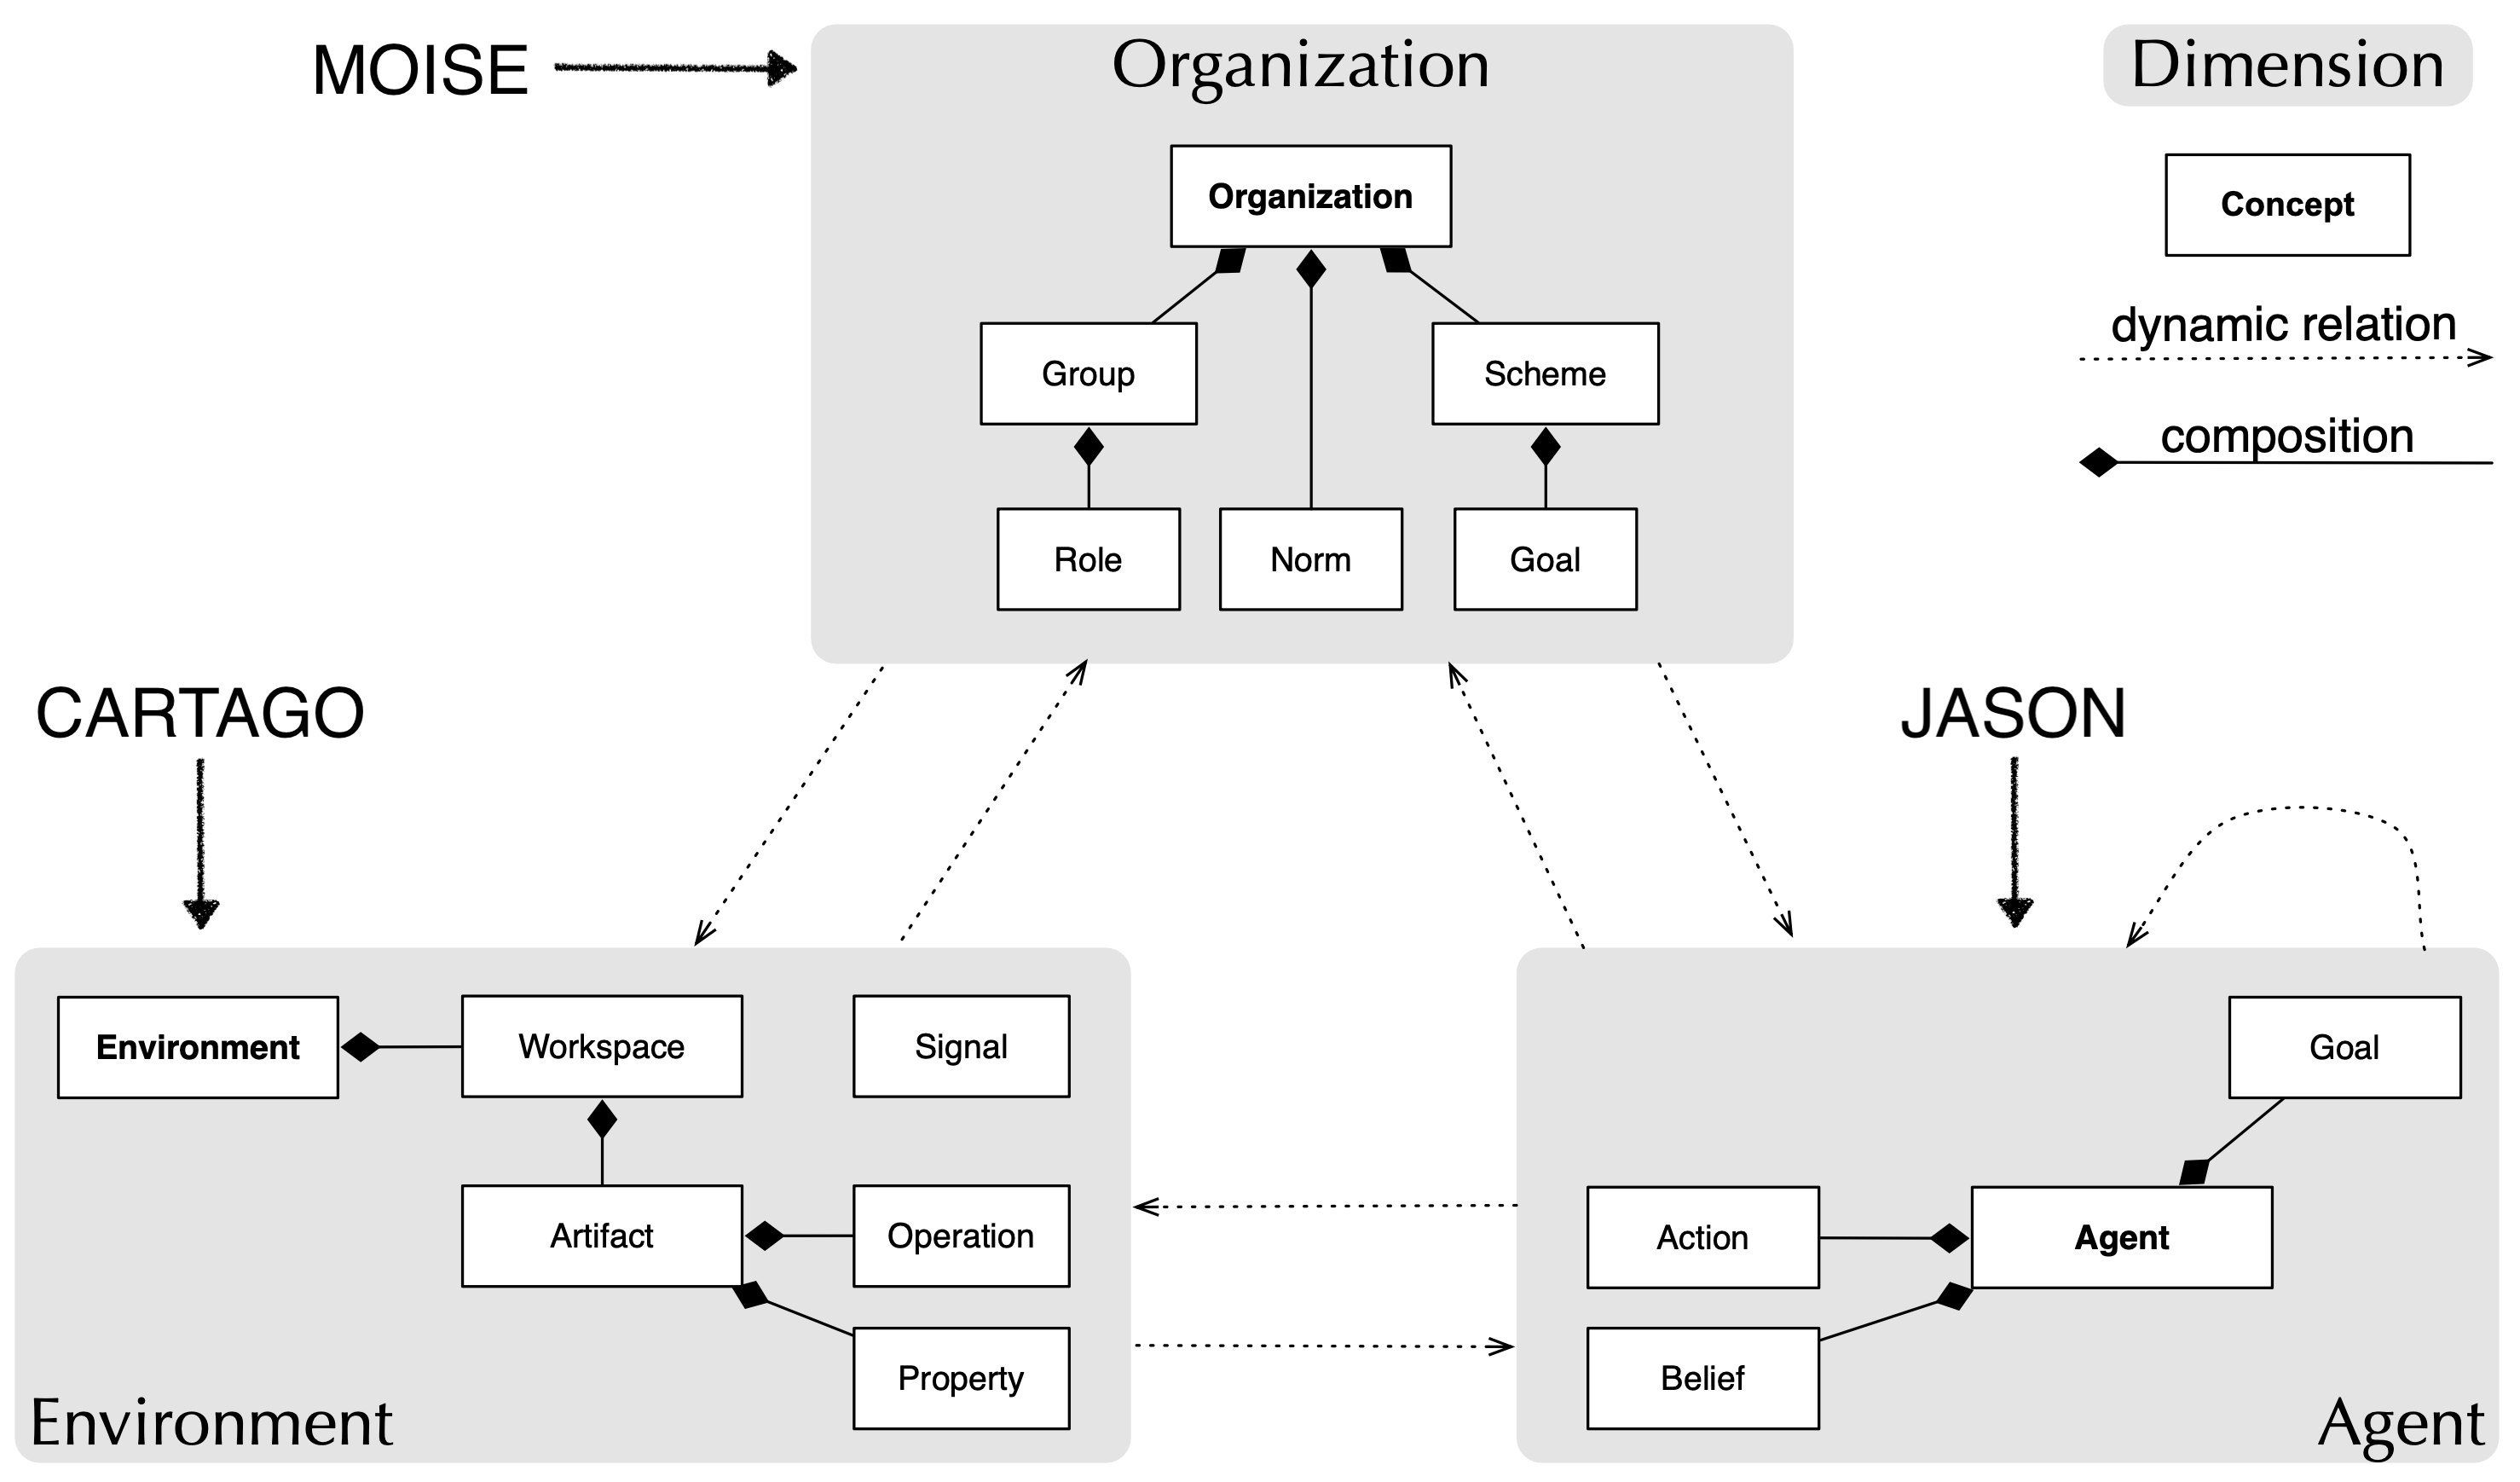
\includegraphics[width=0.9\textwidth]{images/maop.png}
            \end{figure}
        \end{column}
    \end{columns}
\end{frame}

\subsection{Domain Expert Programming}
\begin{frame}{Domain Expert Programming}
    \begin{itemize}
        \item Domain experts are the most suitable for designing solutions for domain-specific problems thanks to their \textbf{expertise}
        \vspace{0.5cm}
        \item The aim is to provide them with user-friendly tools to ground their ideas into a concrete implementation
        \vspace{0.5cm}
        \item Intuitiveness is the key point: the tools should reflect the domain experts' mental model
    \end{itemize}
\end{frame}

\subsection{Visual Programming for MAS}
\begin{frame}{Visual Programming for MAS}
    \begin{columns}
        \begin{column}{0.5\textwidth}
            \begin{itemize}
                \item A block-based visual programming language for agents already exists~\cite{burattini2022agent}\dots
                \item \dots BUT
            \end{itemize}
        \end{column}
        \begin{column}{0.5\textwidth}
            \begin{figure}
                \centering
                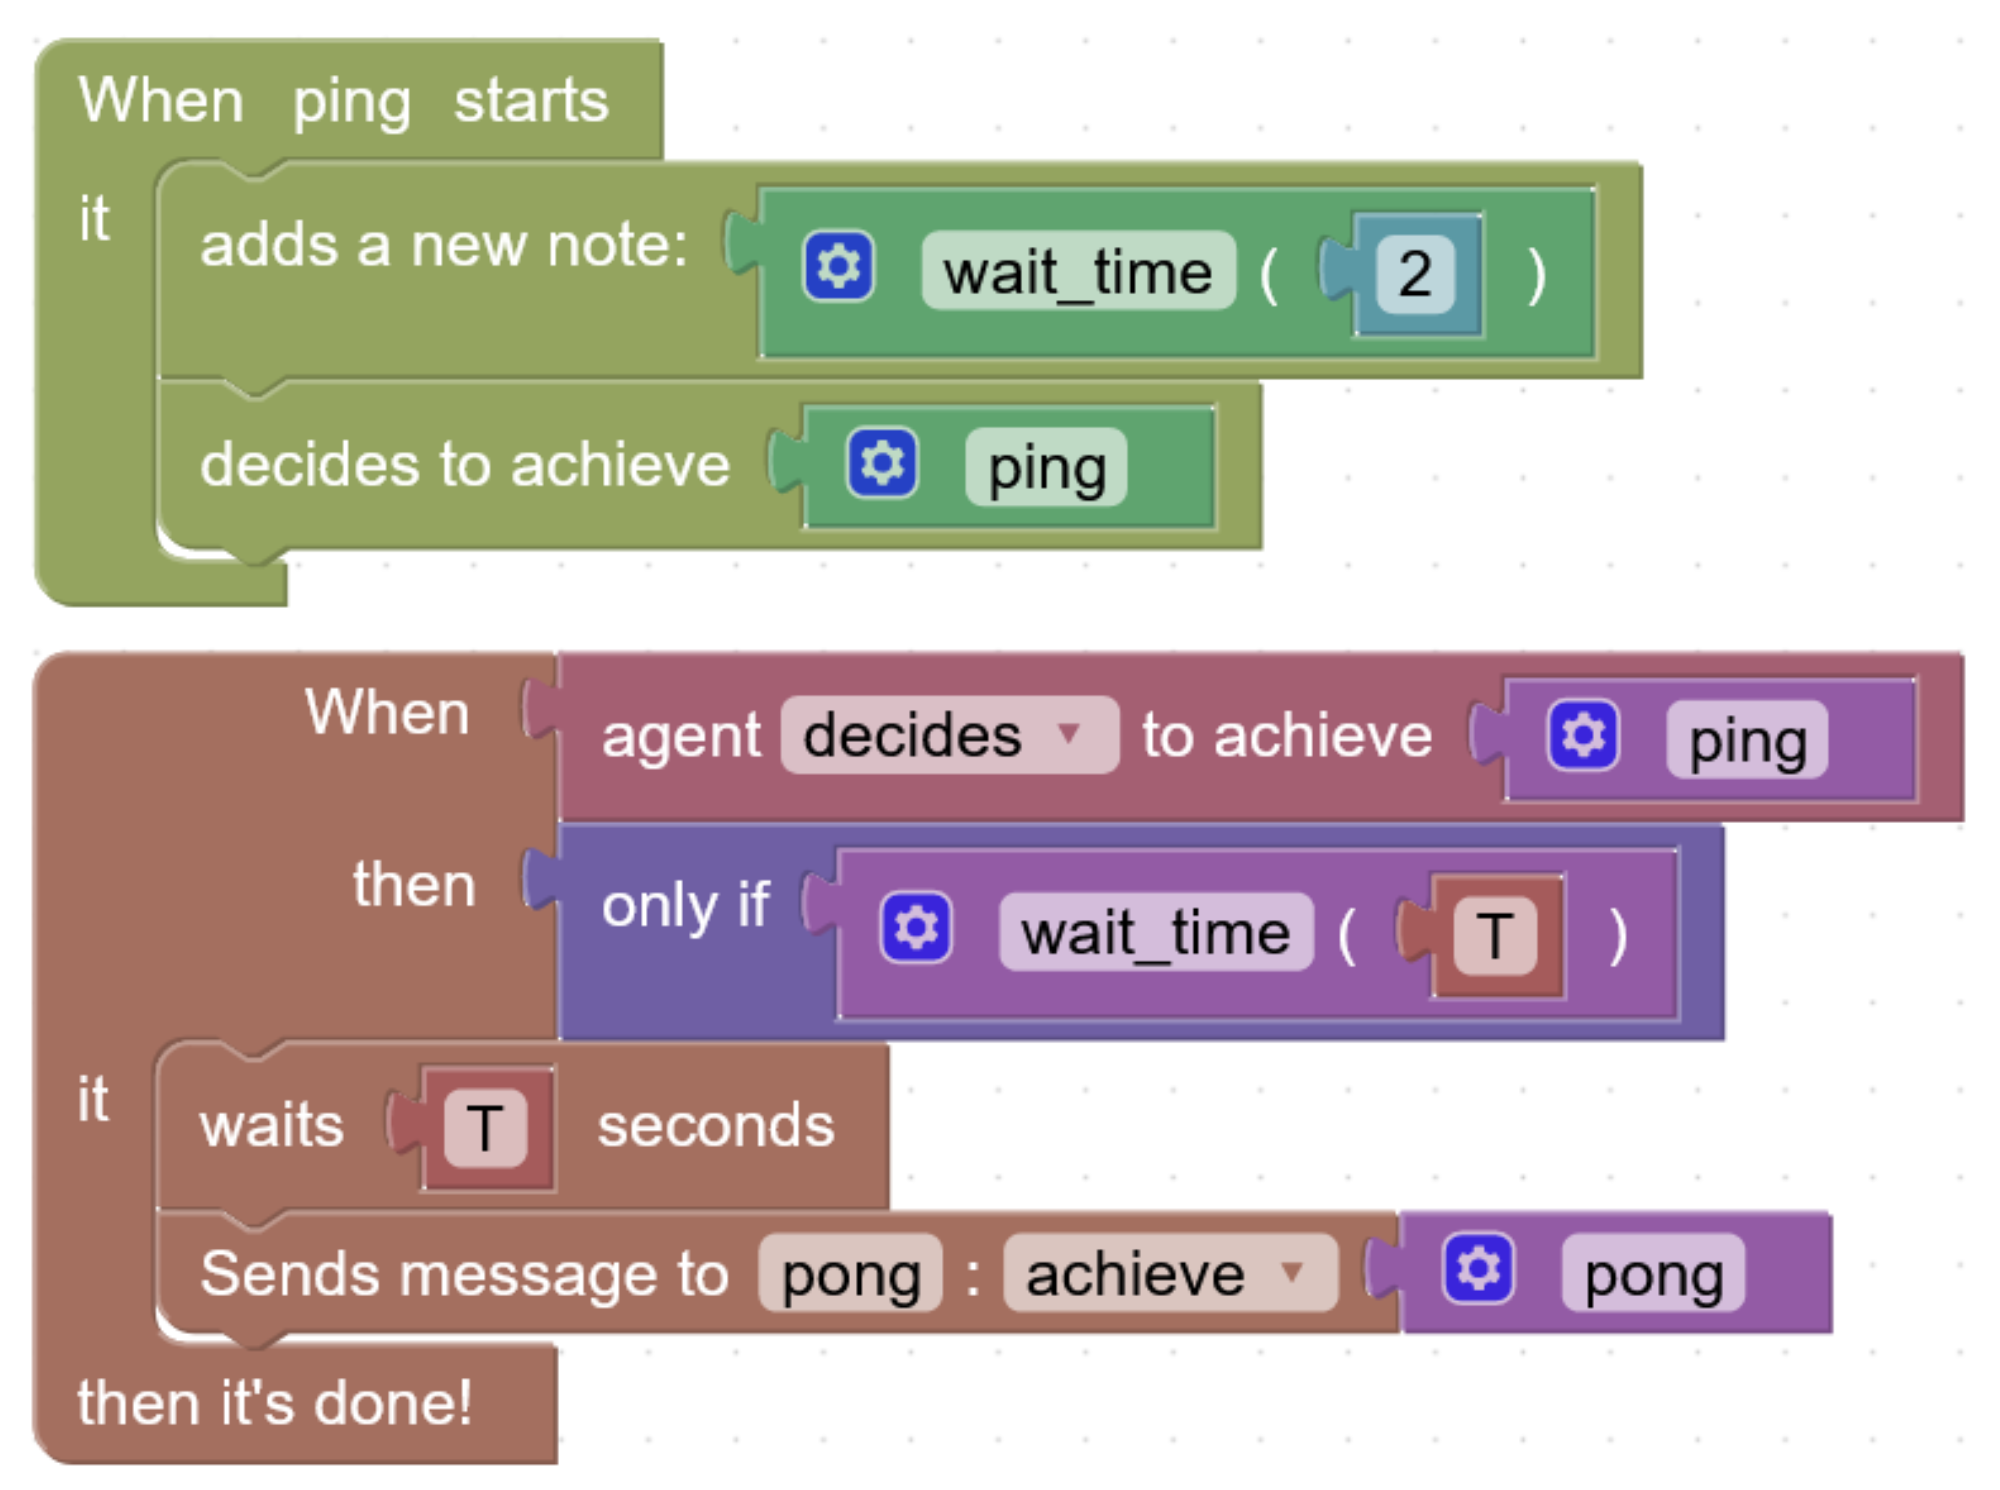
\includegraphics[width=0.9\textwidth]{images/blocks-example.png}
            \end{figure}
        \end{column}
    \end{columns}

    \begin{block}{Challenge}
        Dealing with \textbf{interaction} and \textbf{coordination} between agents in complex systems directly inside the agents makes the design of the system exponentially complex
    \end{block}
\end{frame}

\section{Problem Analysis}
\begin{frame}{Objectives of the Thesis}
    \begin{block}{Goal}
        Provide users with a way to intuitively define MAS \textbf{organizations}
    \end{block}
    
    \begin{exampleblock}{Key Points}
        \begin{itemize}
            \item Design of a \textbf{visual language} capable of defining:
            \begin{itemize}
                \item the \emph{structure}
                \item the \emph{behavior}
                \item the \emph{norms}
            \end{itemize}
            of the organization
            \item Implementation of a Web-based, easy-to-use \textbf{development environment}
            \item Integration with the \textit{agents runtime environment} to \textbf{deploy} and \textbf{enforce} organizations
        \end{itemize}
    \end{exampleblock}
\end{frame}


\section{Design}

\subsection{The Visual Language}
\begin{frame}[allowframebreaks]{The Visual Language}
\begin{itemize}
    \vspace{-0.5cm}
    \item The analysis of \moise{} and the creation of a focus group brought to the following design
    \vspace{0.5cm}
    \item Building blocks of the organization's \textbf{structure}:
\end{itemize}

\begin{columns}
    \begin{column}{0.5\textwidth}
        \begin{figure}
            \centering
            
\includegraphics[width=0.35\textwidth]{images/visual-language/concrete-role.png}
        \end{figure}
    \end{column}
    \begin{column}{0.5\textwidth}
        \begin{figure}
            \centering
            
\includegraphics[width=0.35\textwidth]{images/visual-language/abstract-role.png}
        \end{figure}
    \end{column}
\end{columns}

\begin{columns}
    \begin{column}{0.5\textwidth}
        \begin{figure}
            \centering
            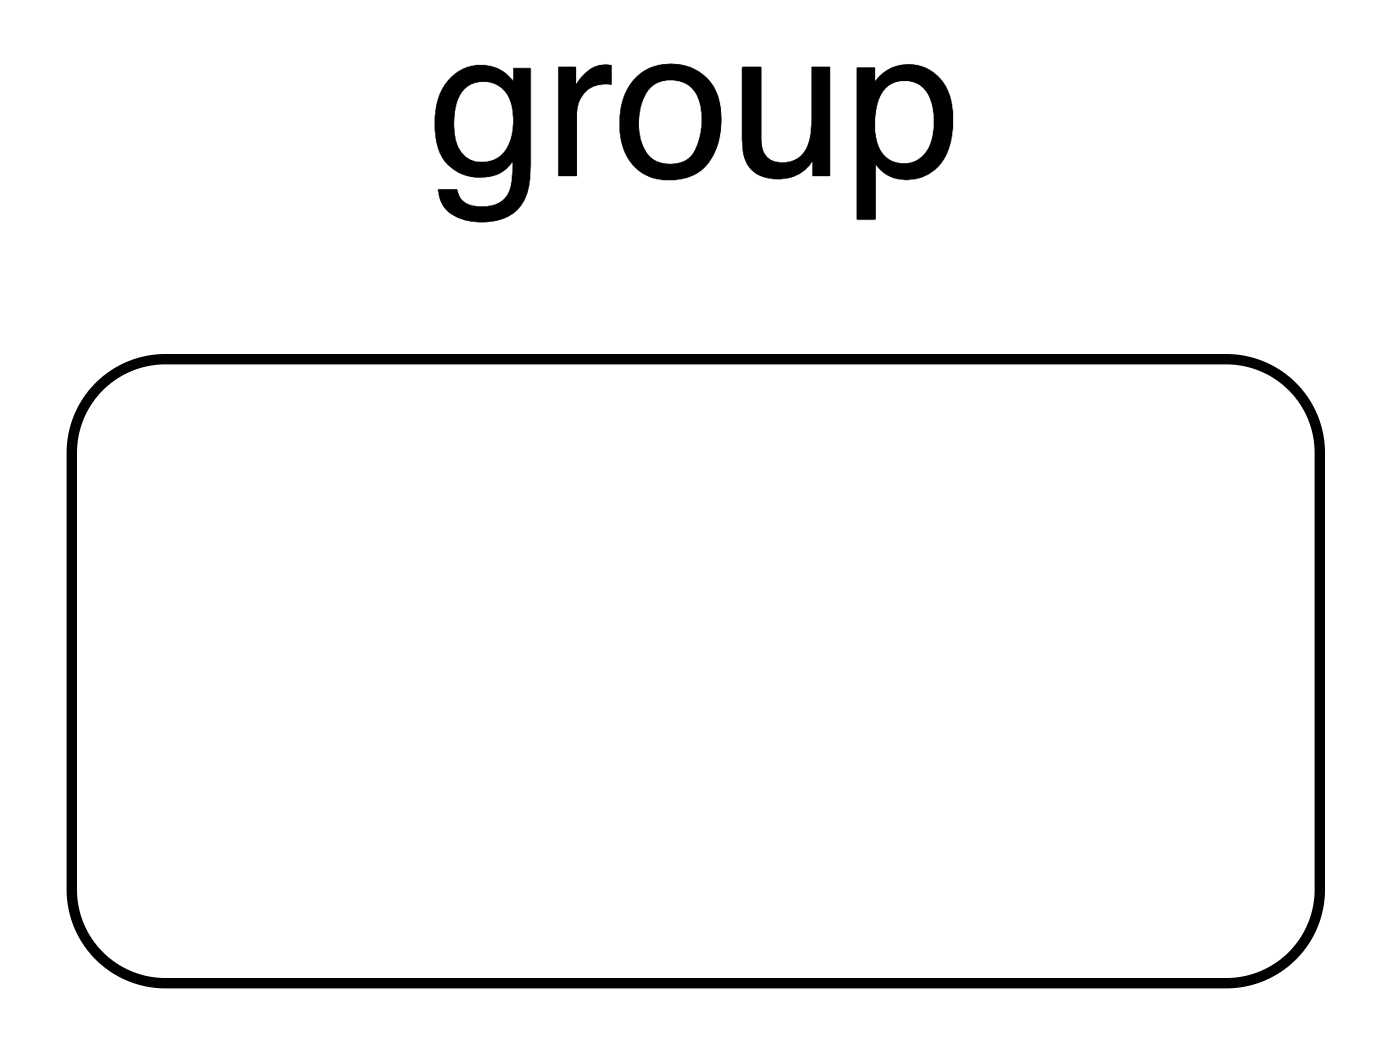
\includegraphics[width=0.35\textwidth]{images/visual-language/group.png}
        \end{figure}
    \end{column}
    \begin{column}{0.25\textwidth}
        \begin{figure}
            \centering
            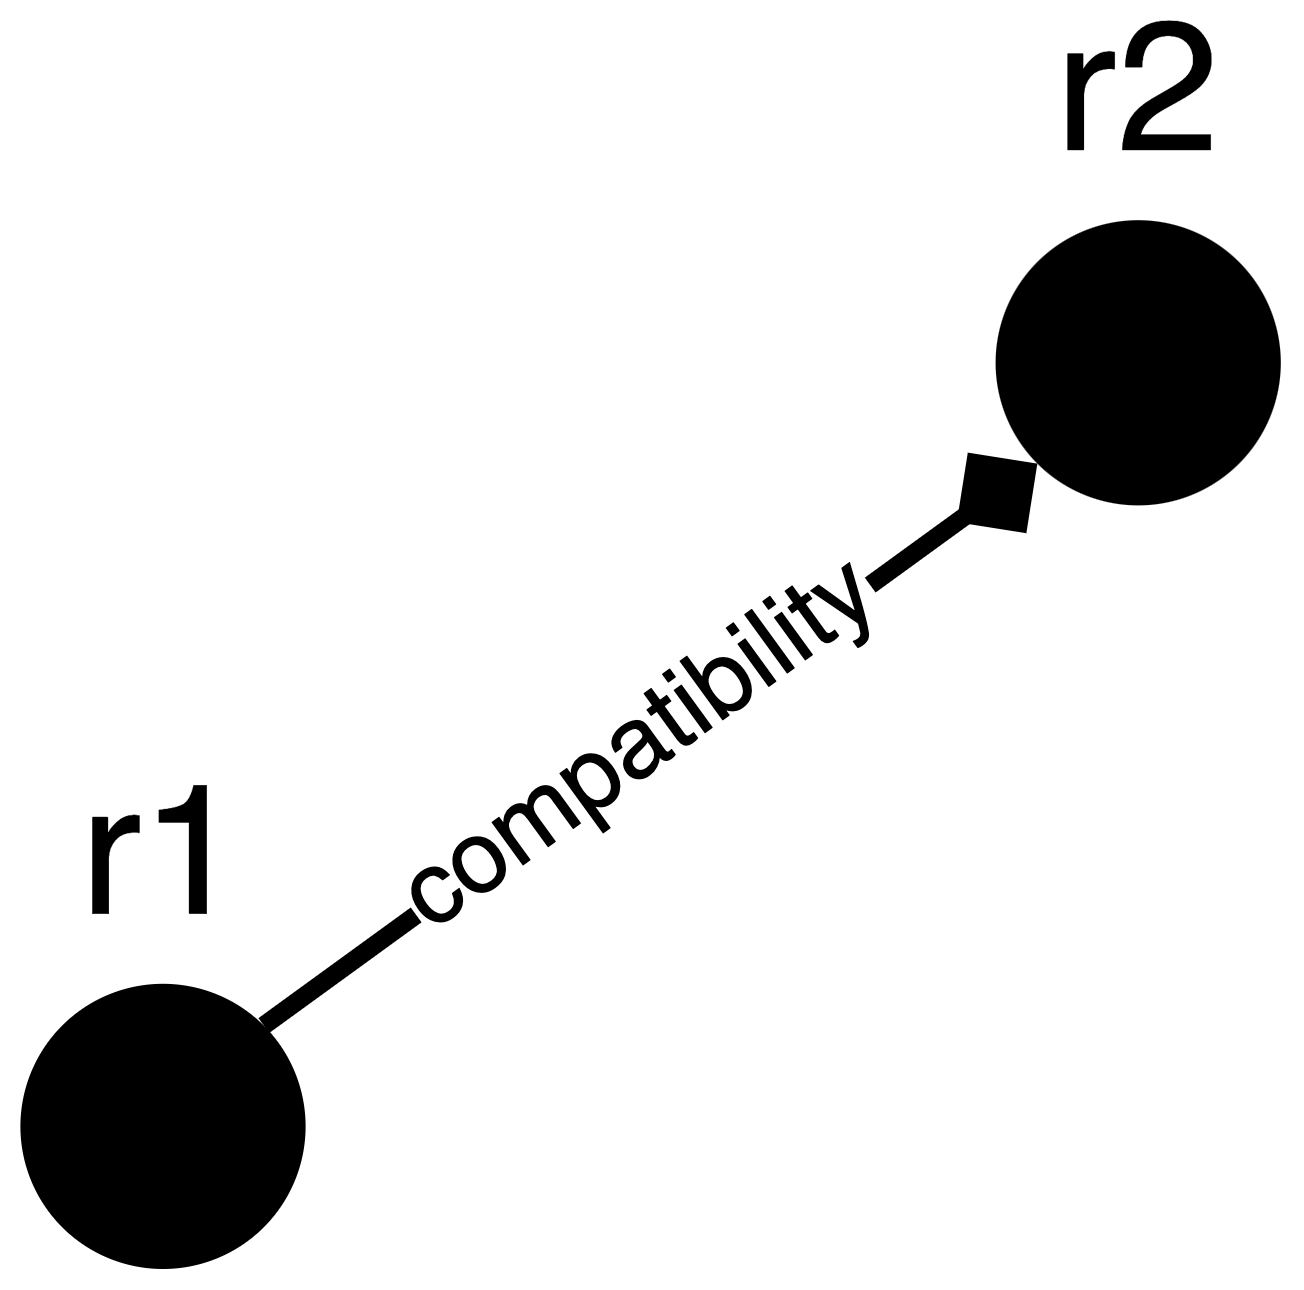
\includegraphics[width=0.7\textwidth]{images/visual-language/compatibility.png}
        \end{figure}
    \end{column}
    \begin{column}{0.25\textwidth}
        \begin{figure}
            \centering
            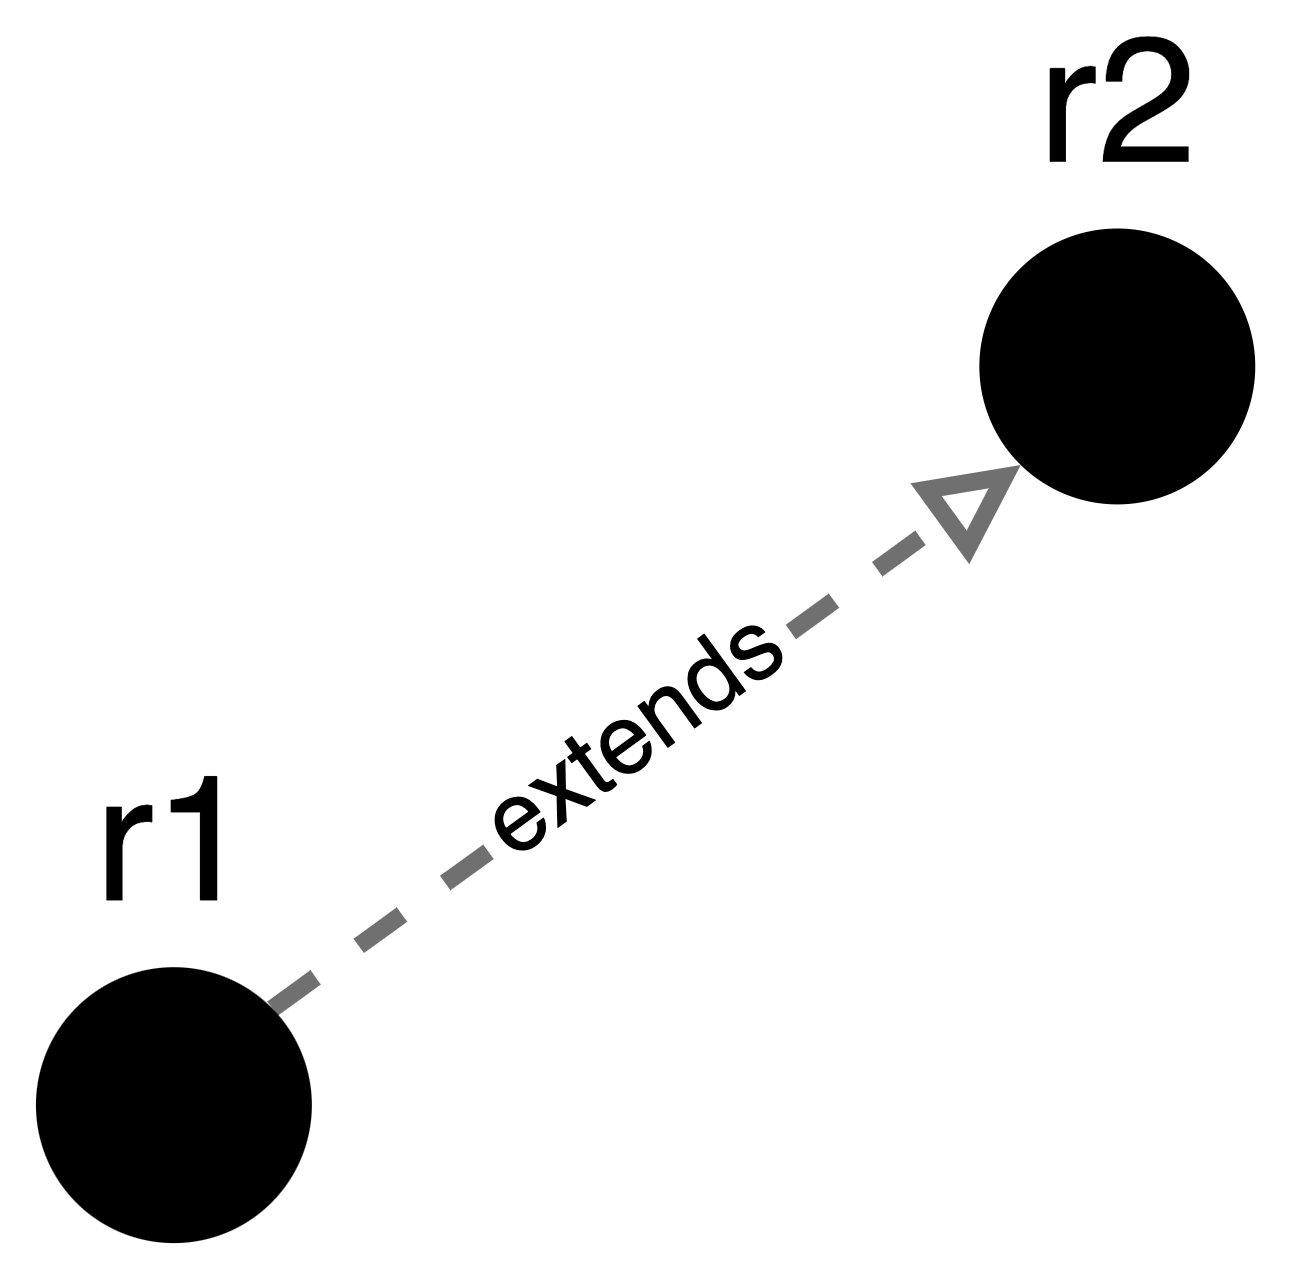
\includegraphics[width=0.7\textwidth]{images/visual-language/extension.png}
        \end{figure}
    \end{column}
\end{columns}

\framebreak

\begin{itemize}
    \vspace{-0.5cm}
    \item The analysis of \moise{} and the creation of a focus group brought to the following design
    \vspace{0.5cm}
    \item Building blocks of the organization's \textbf{behavior}:
\end{itemize}

\begin{columns}
    \begin{column}{0.5\textwidth}
        \begin{figure}
            \centering
            
\includegraphics[width=0.35\textwidth]{images/visual-language/goal.png}
        \end{figure}
    \end{column}
    \begin{column}{0.5\textwidth}
        \begin{figure}
            \centering
            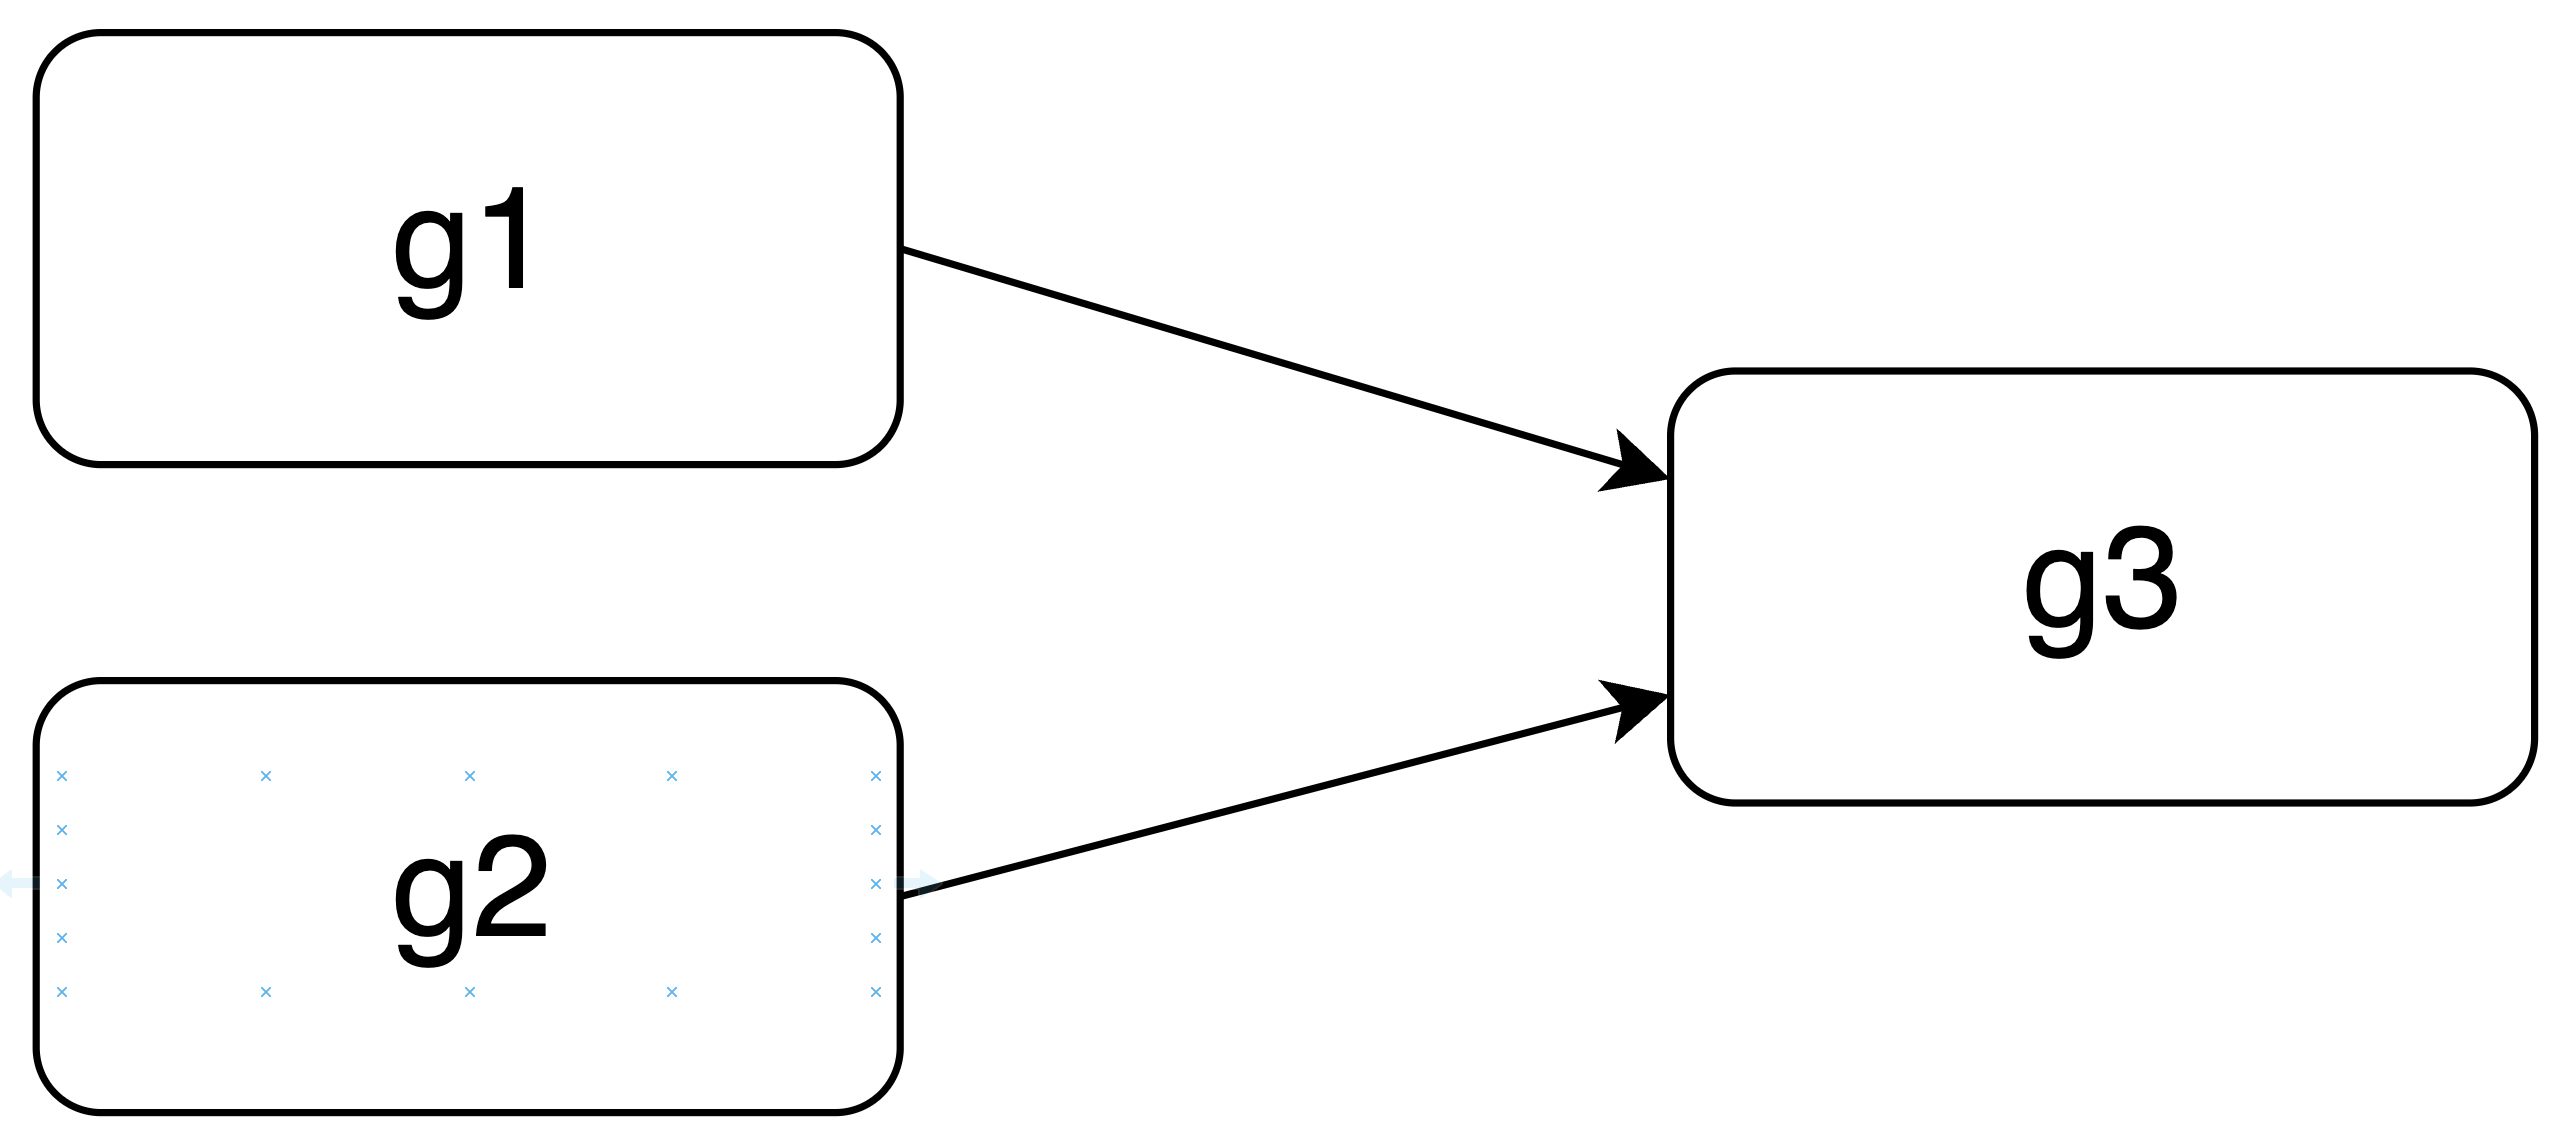
\includegraphics[width=0.7\textwidth]{images/visual-language/dependency-and.png}
        \end{figure}
    \end{column}
\end{columns}

\begin{columns}
    \begin{column}{0.5\textwidth}
        \begin{figure}
            \centering
            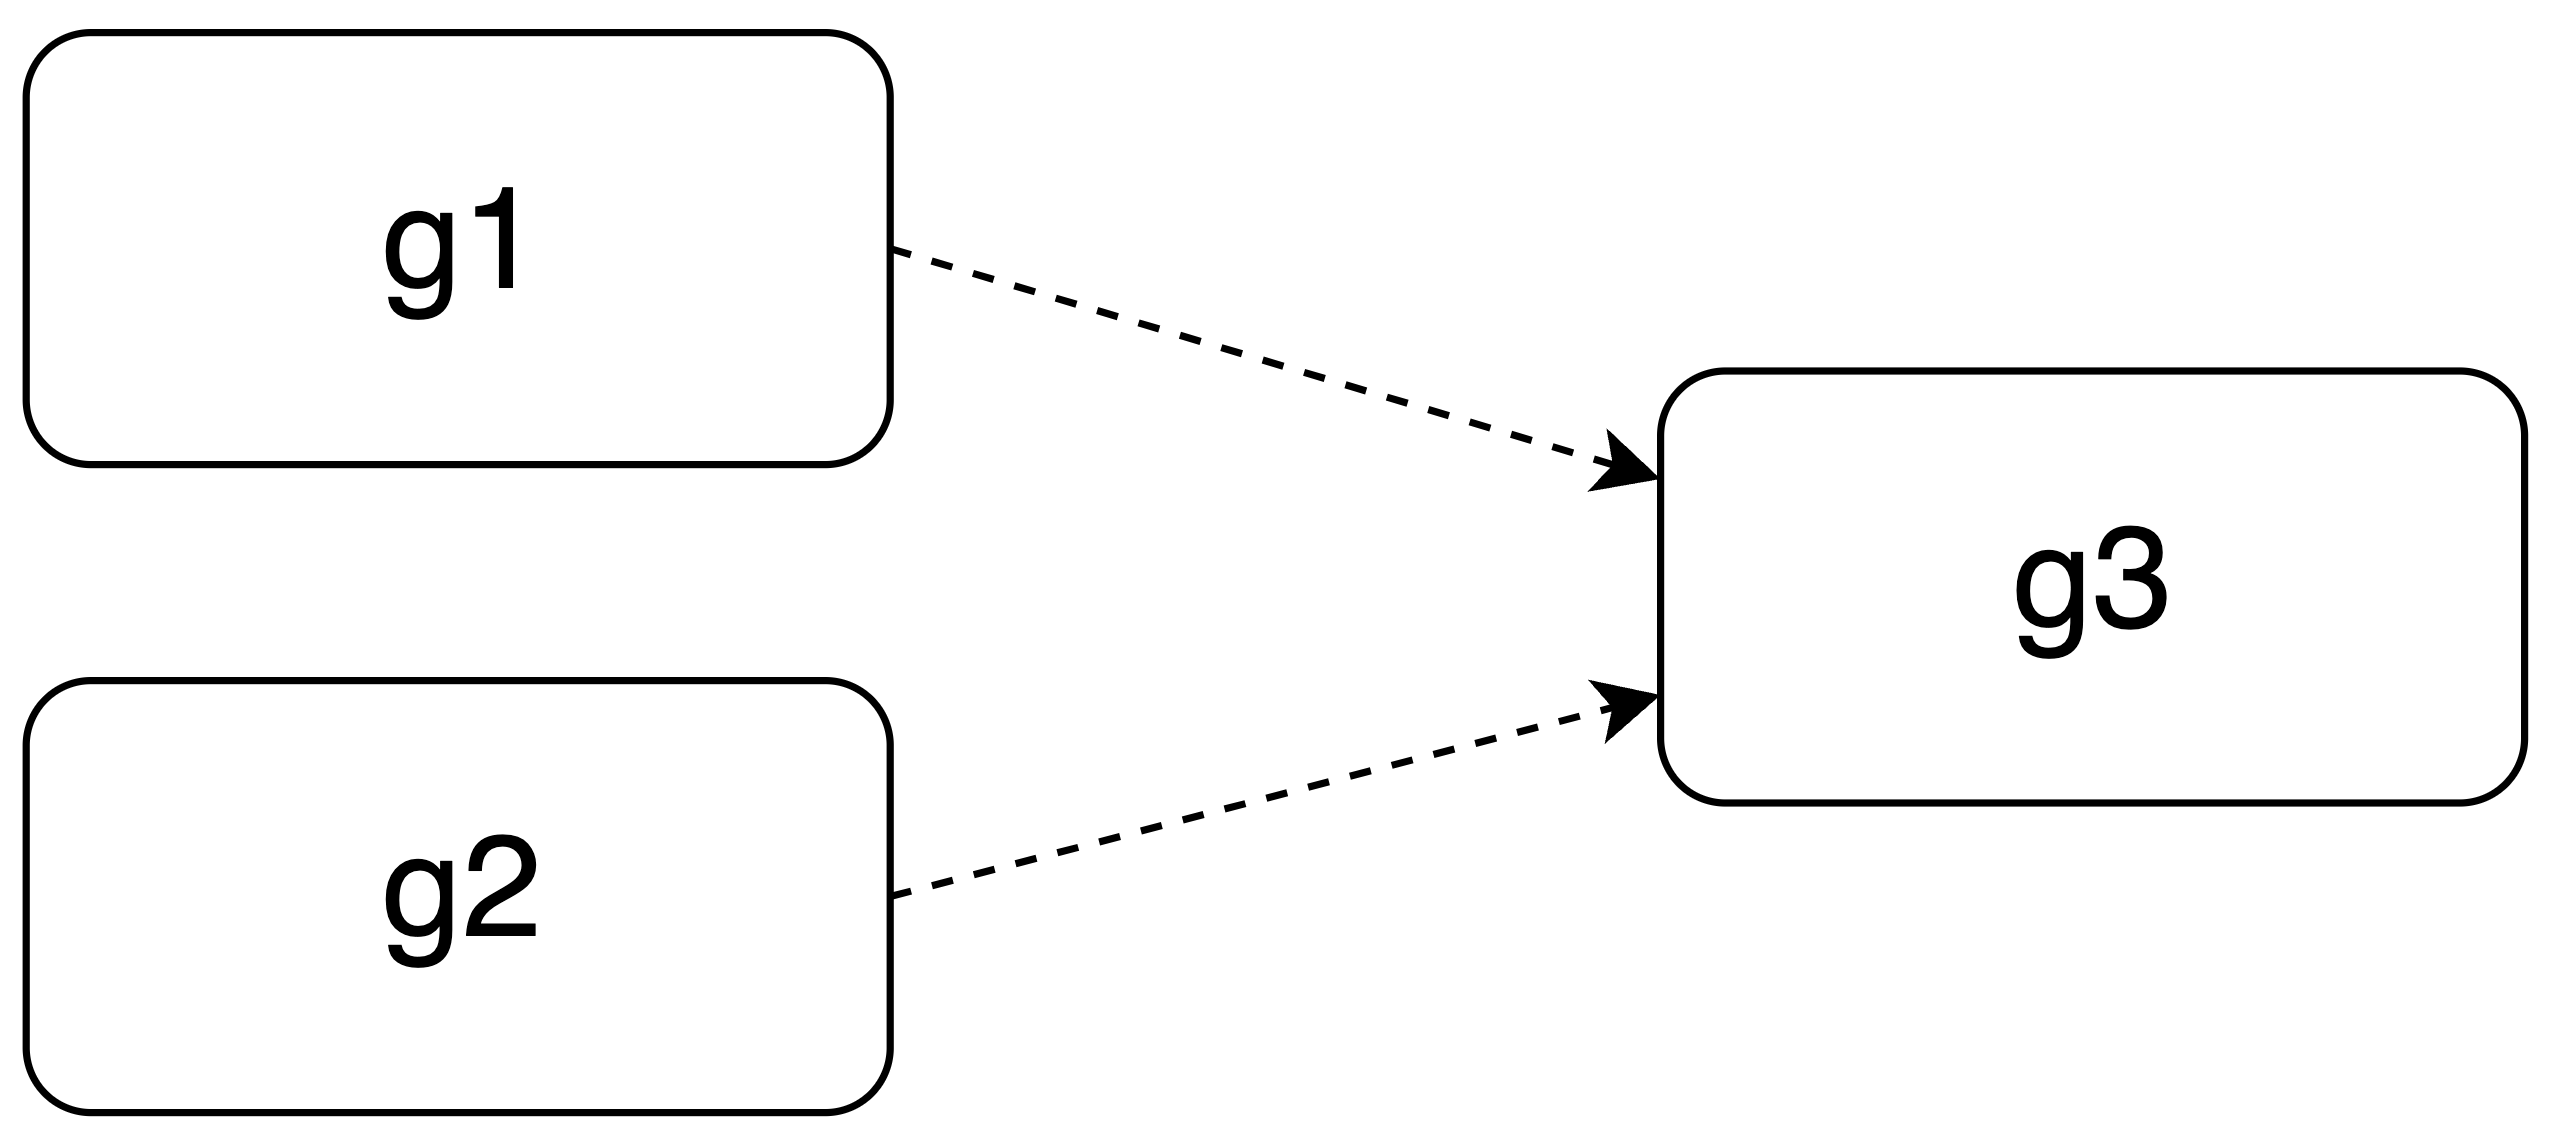
\includegraphics[width=0.7\textwidth]{images/visual-language/dependency-or.png}
        \end{figure}
    \end{column}
    \begin{column}{0.5\textwidth}
        \begin{figure}
            \centering
            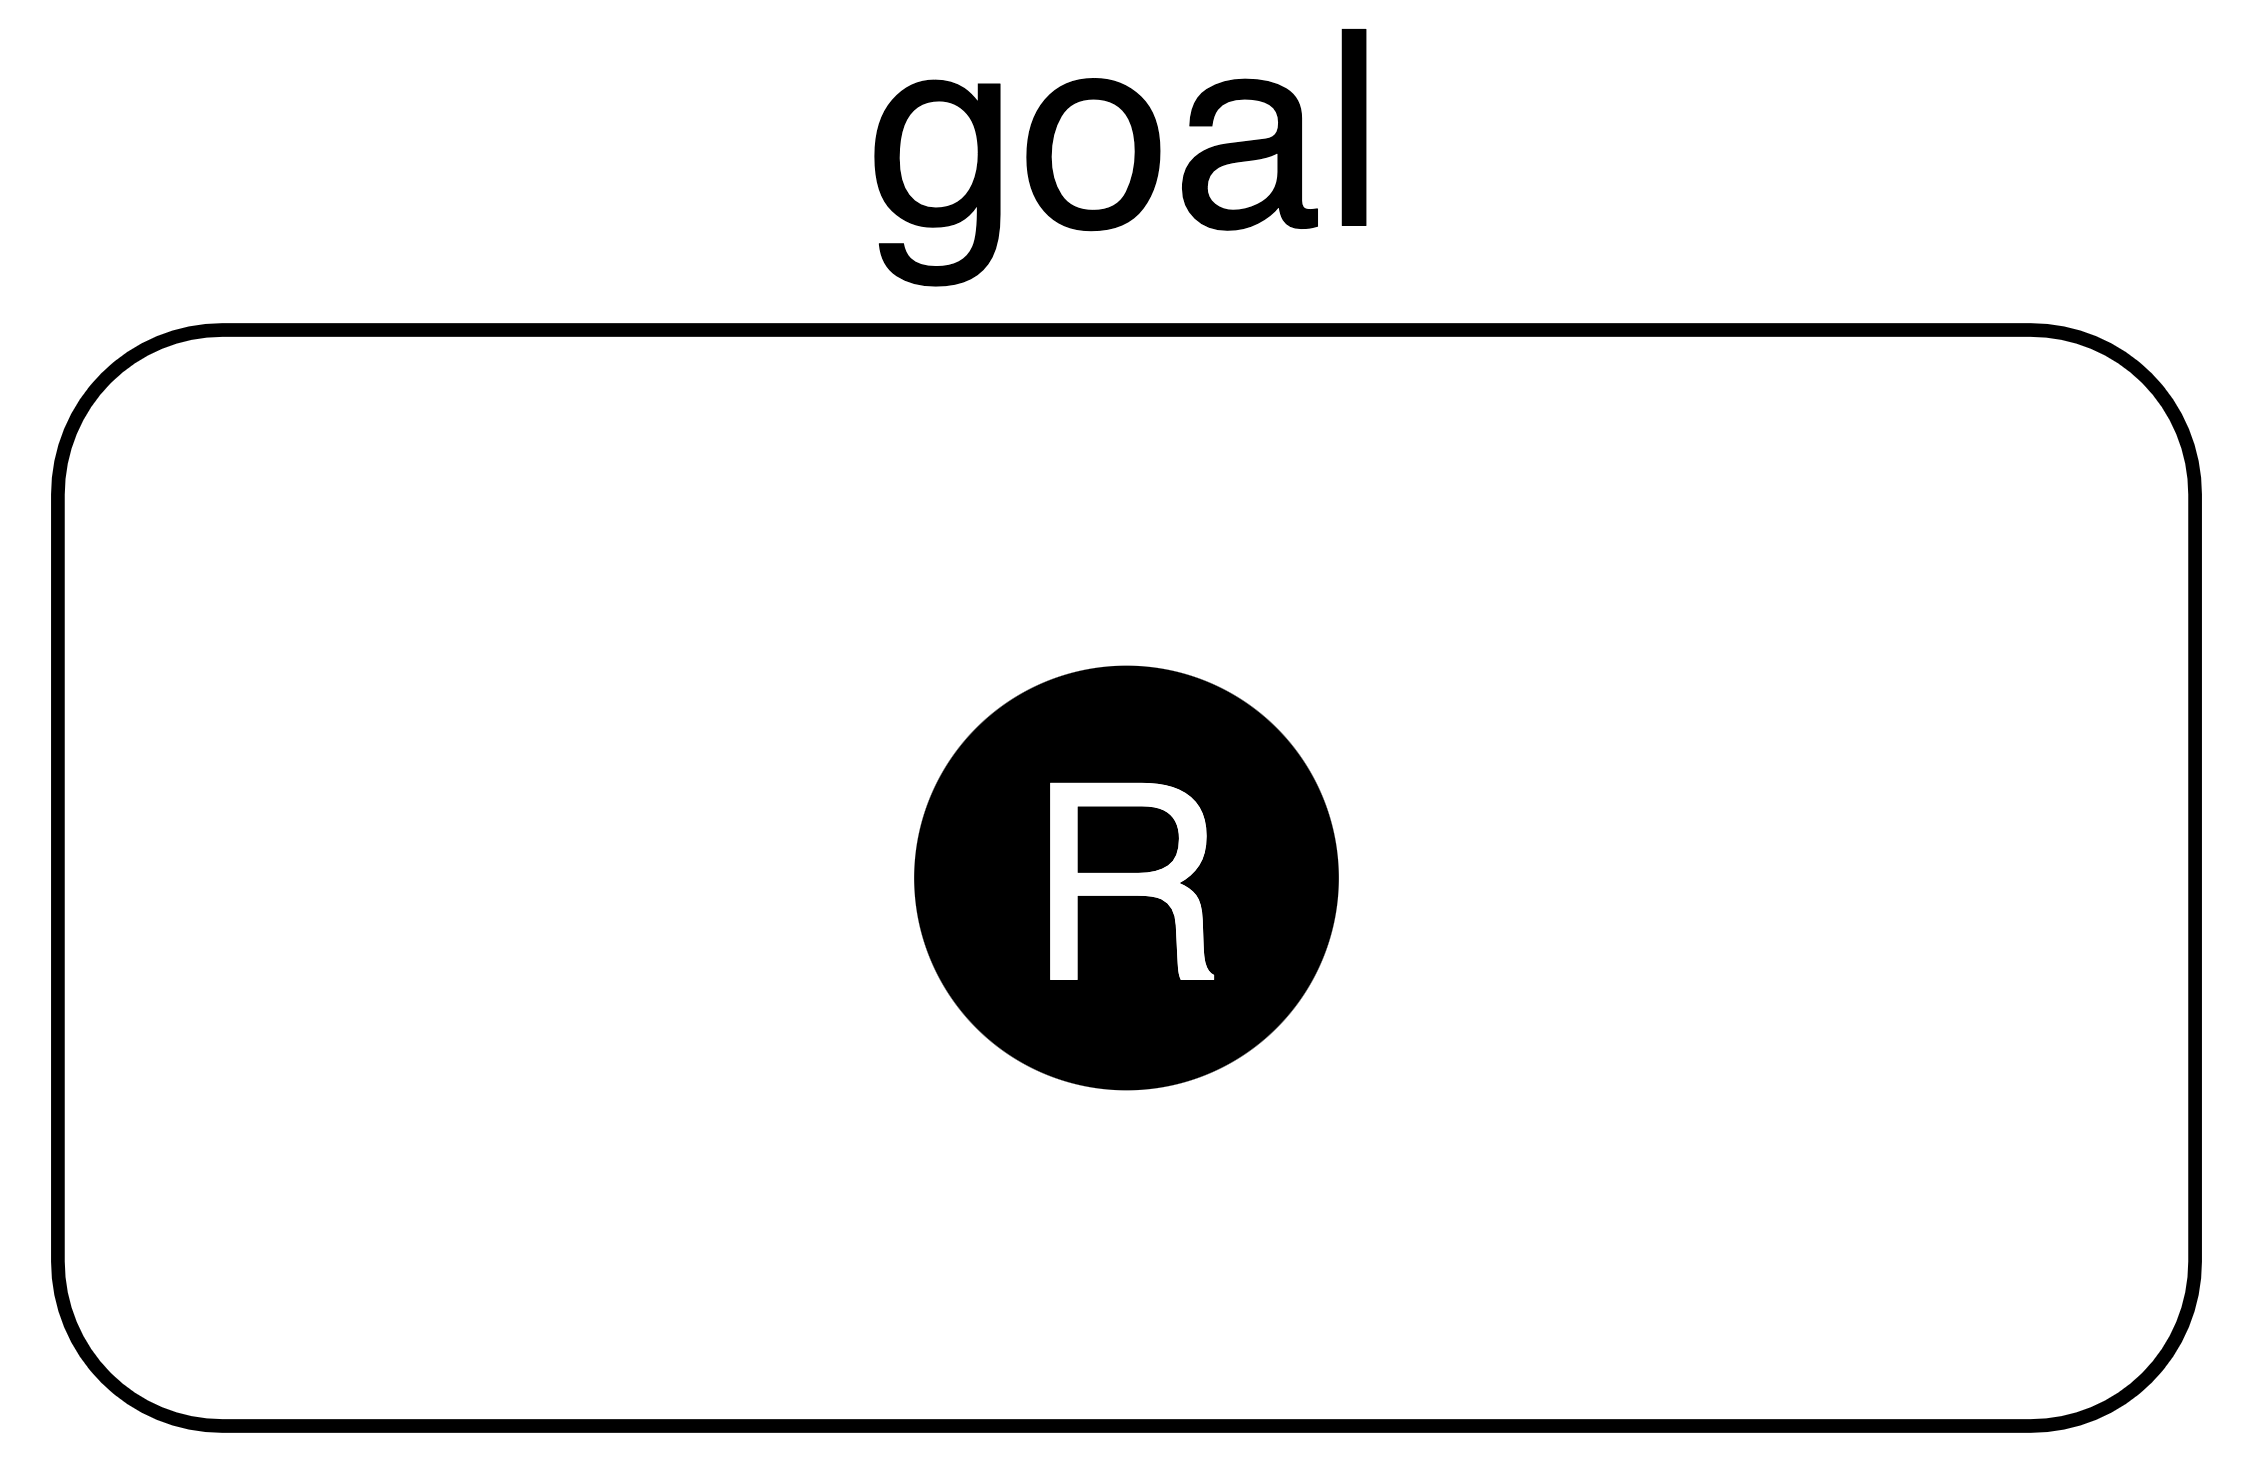
\includegraphics[width=0.35\textwidth]{images/visual-language/goal-allocation.png}
        \end{figure}
    \end{column}
\end{columns}

\end{frame}

\subsection{The Development Environment}
\begin{frame}[allowframebreaks]{The Development Environment}
    \hspace{-0.5cm}
    \begin{tikzpicture}
        \node (structural){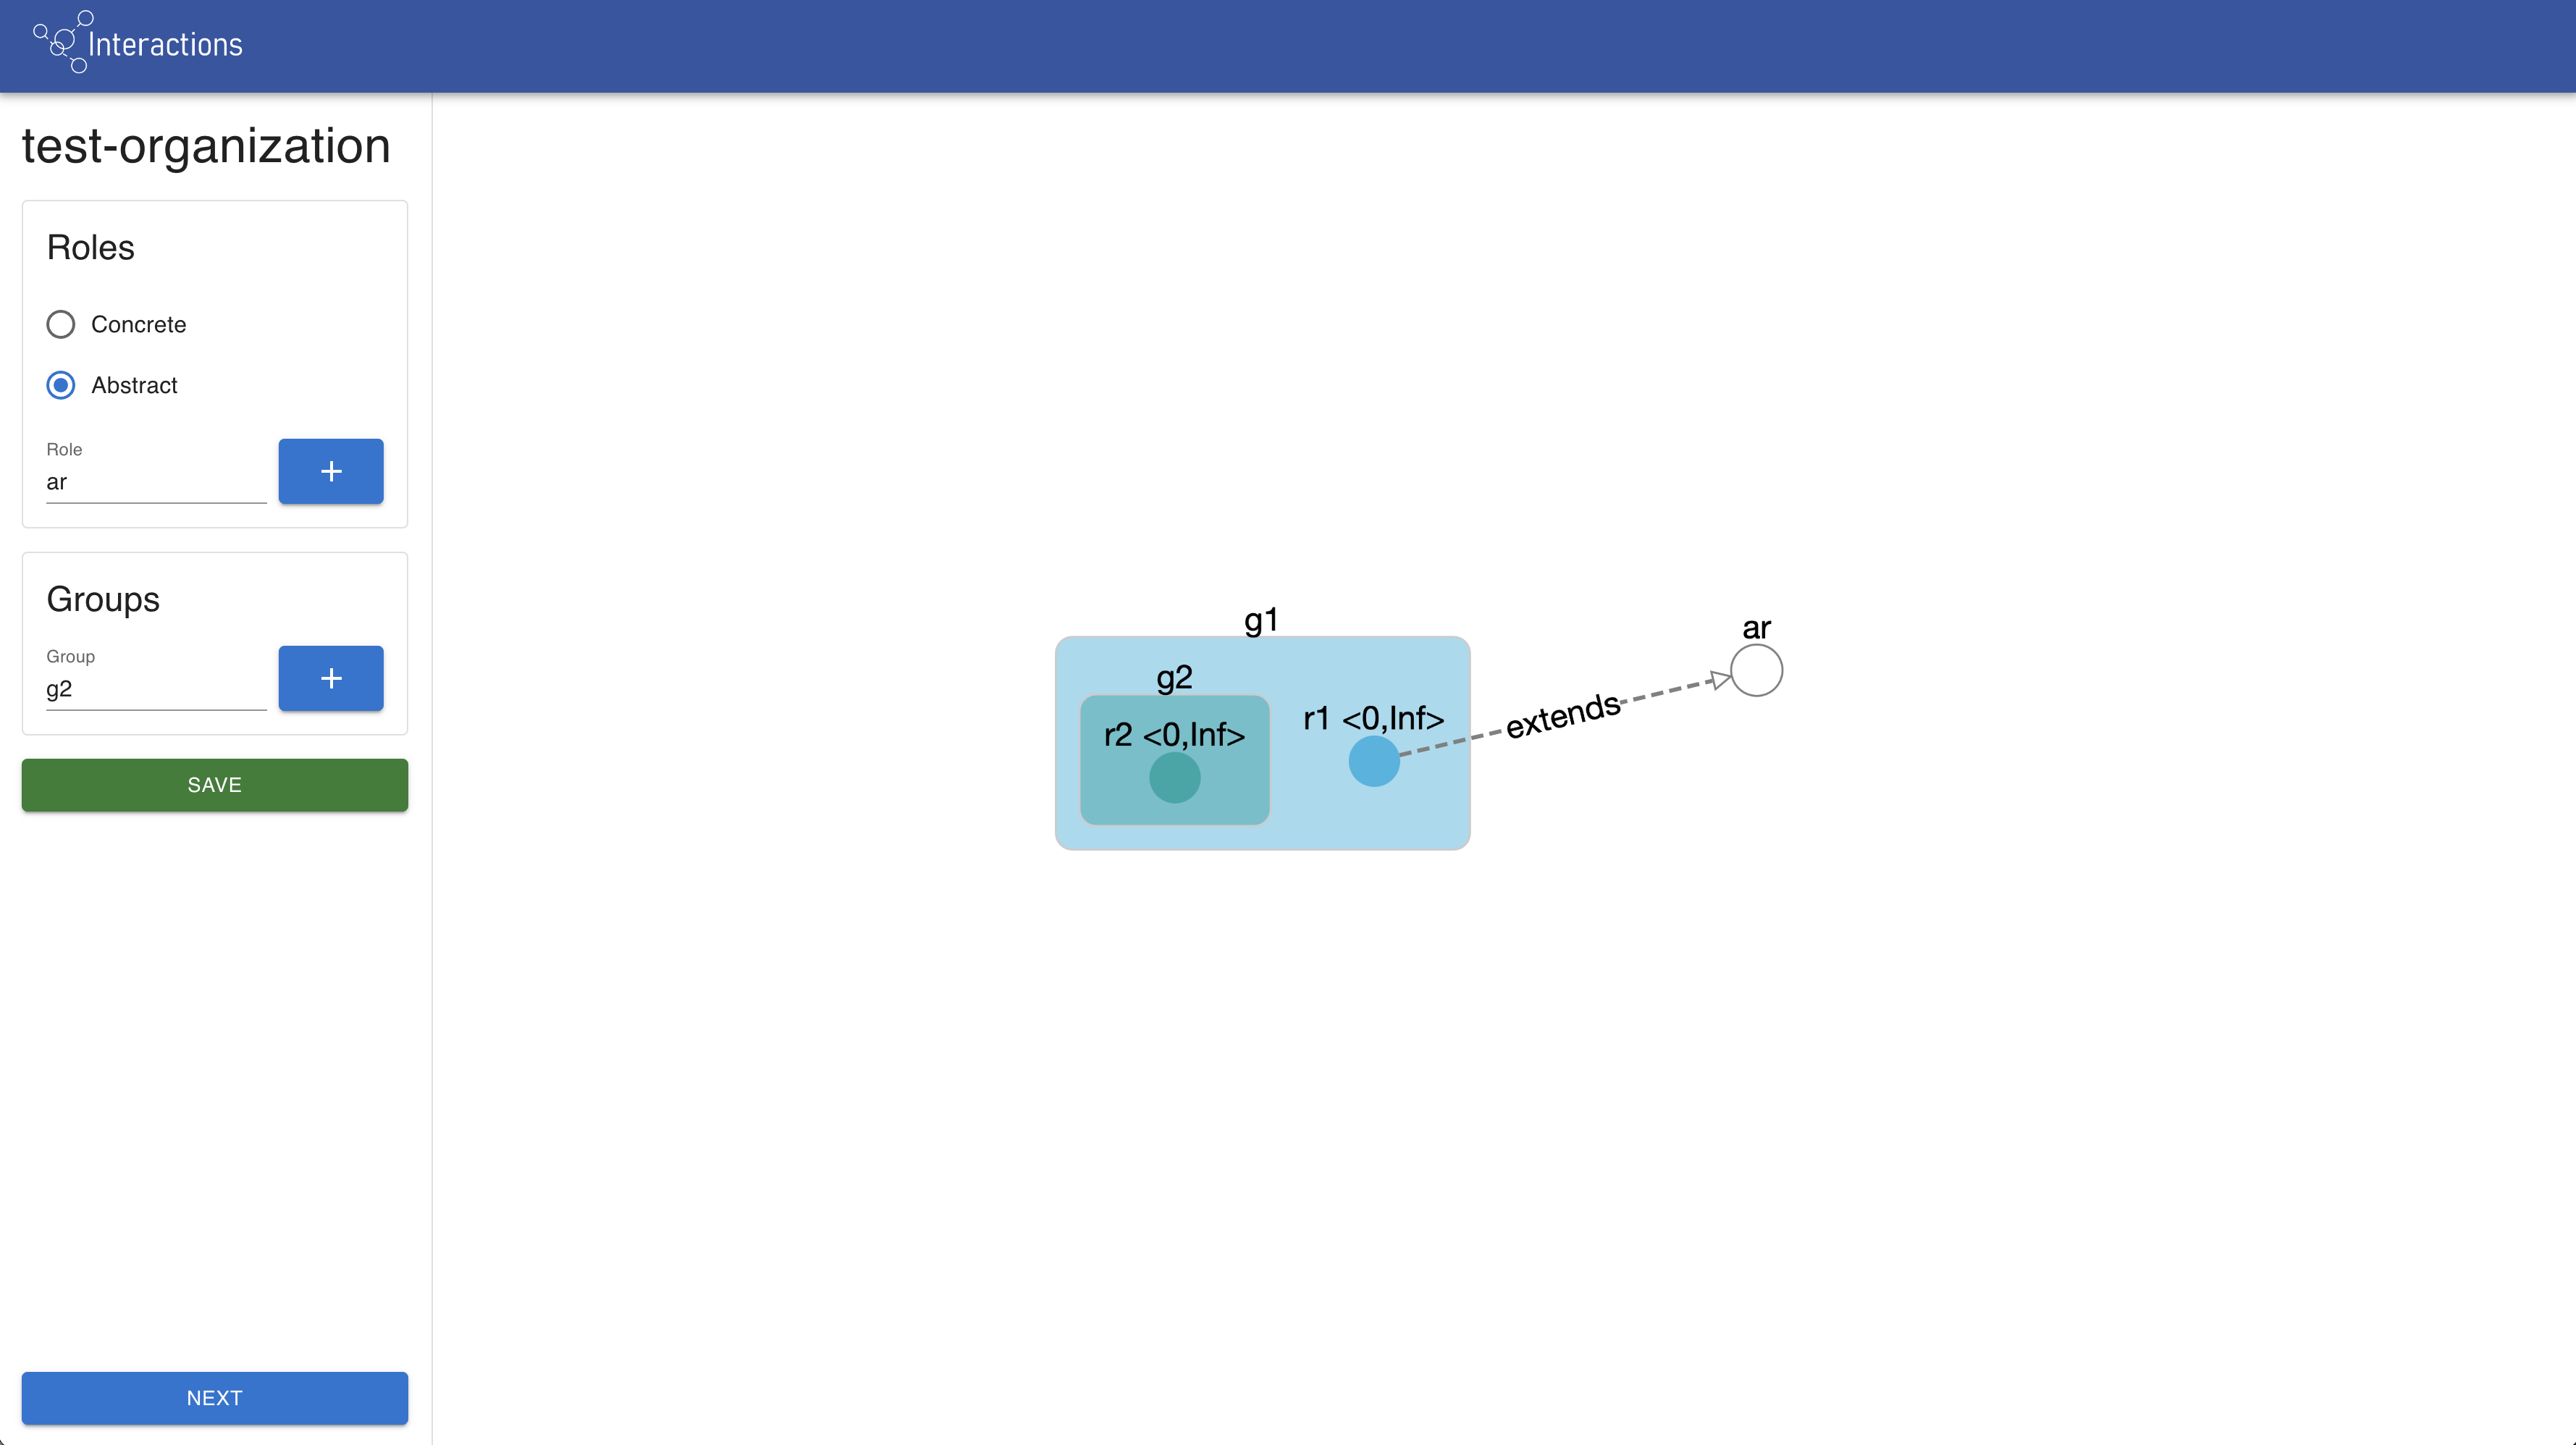
\includegraphics[height=4.2cm]{images/ide/structural.png}};
        \node (structural-side) at (structural.south east)[xshift=0.8cm,yshift=-0.5cm] {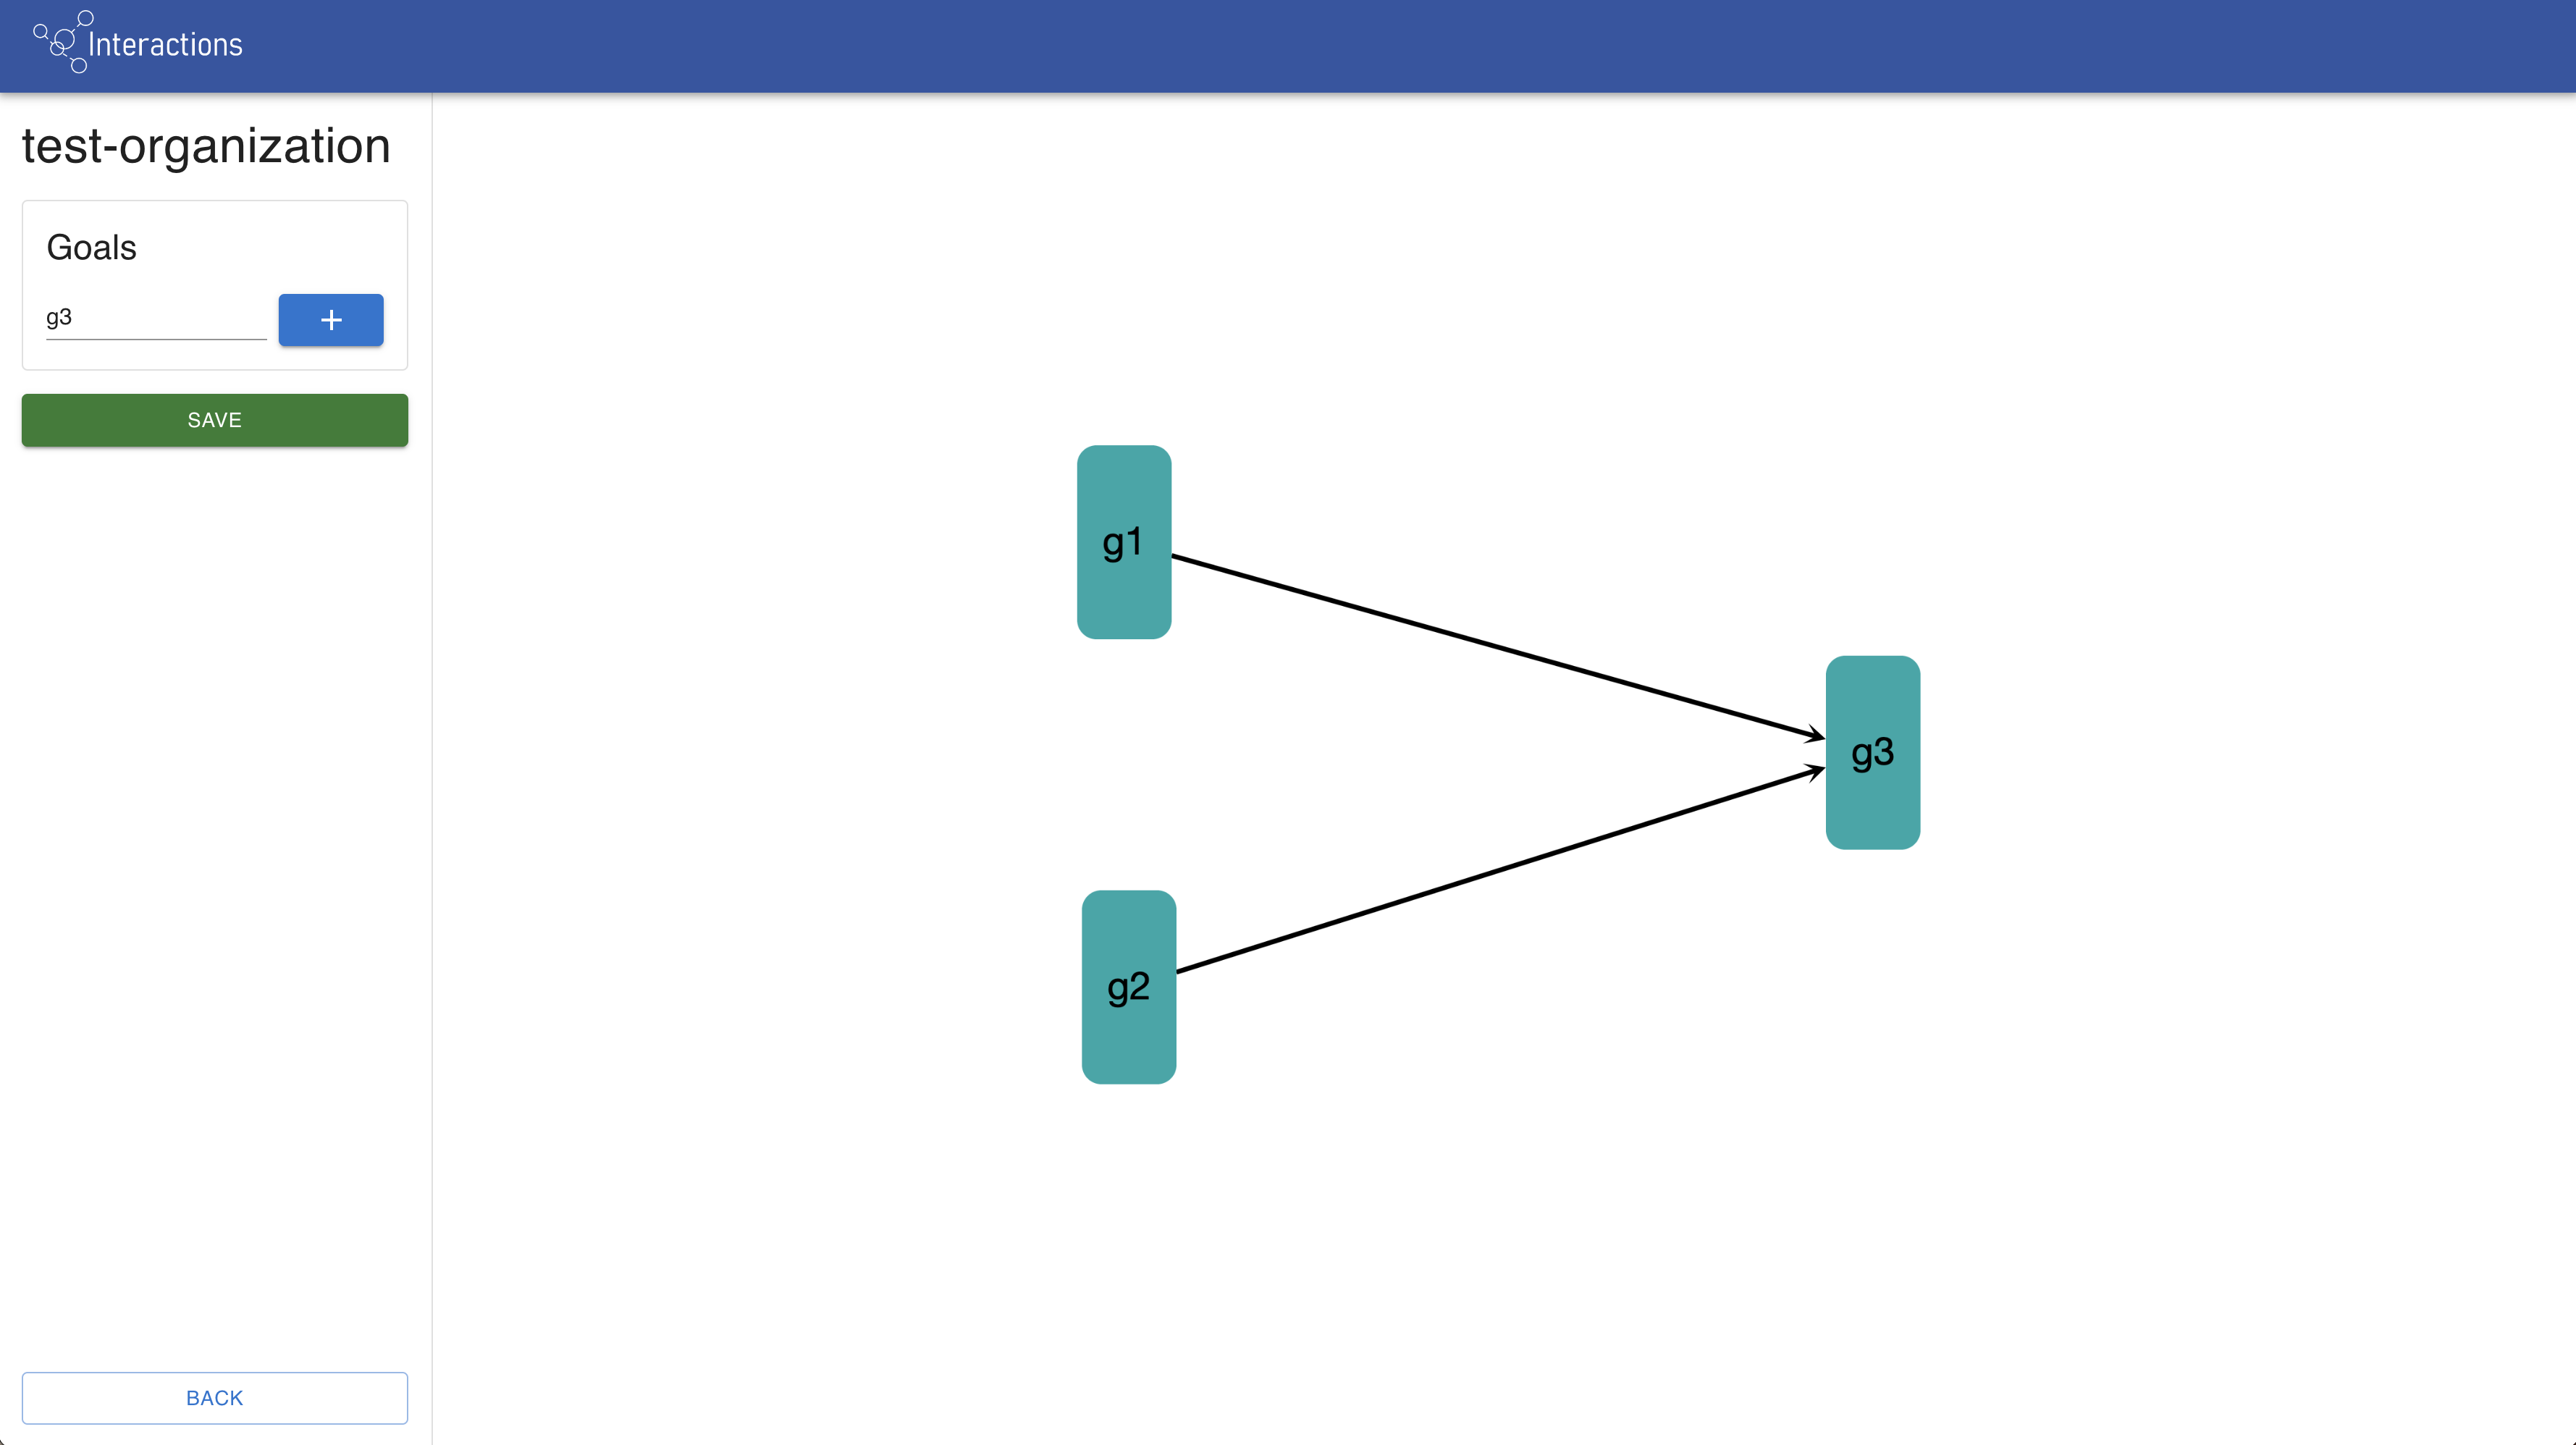
\includegraphics[height=4.2cm]{images/ide/functional.png}};
    \end{tikzpicture}

    \framebreak

    \begin{figure}
        \centering
        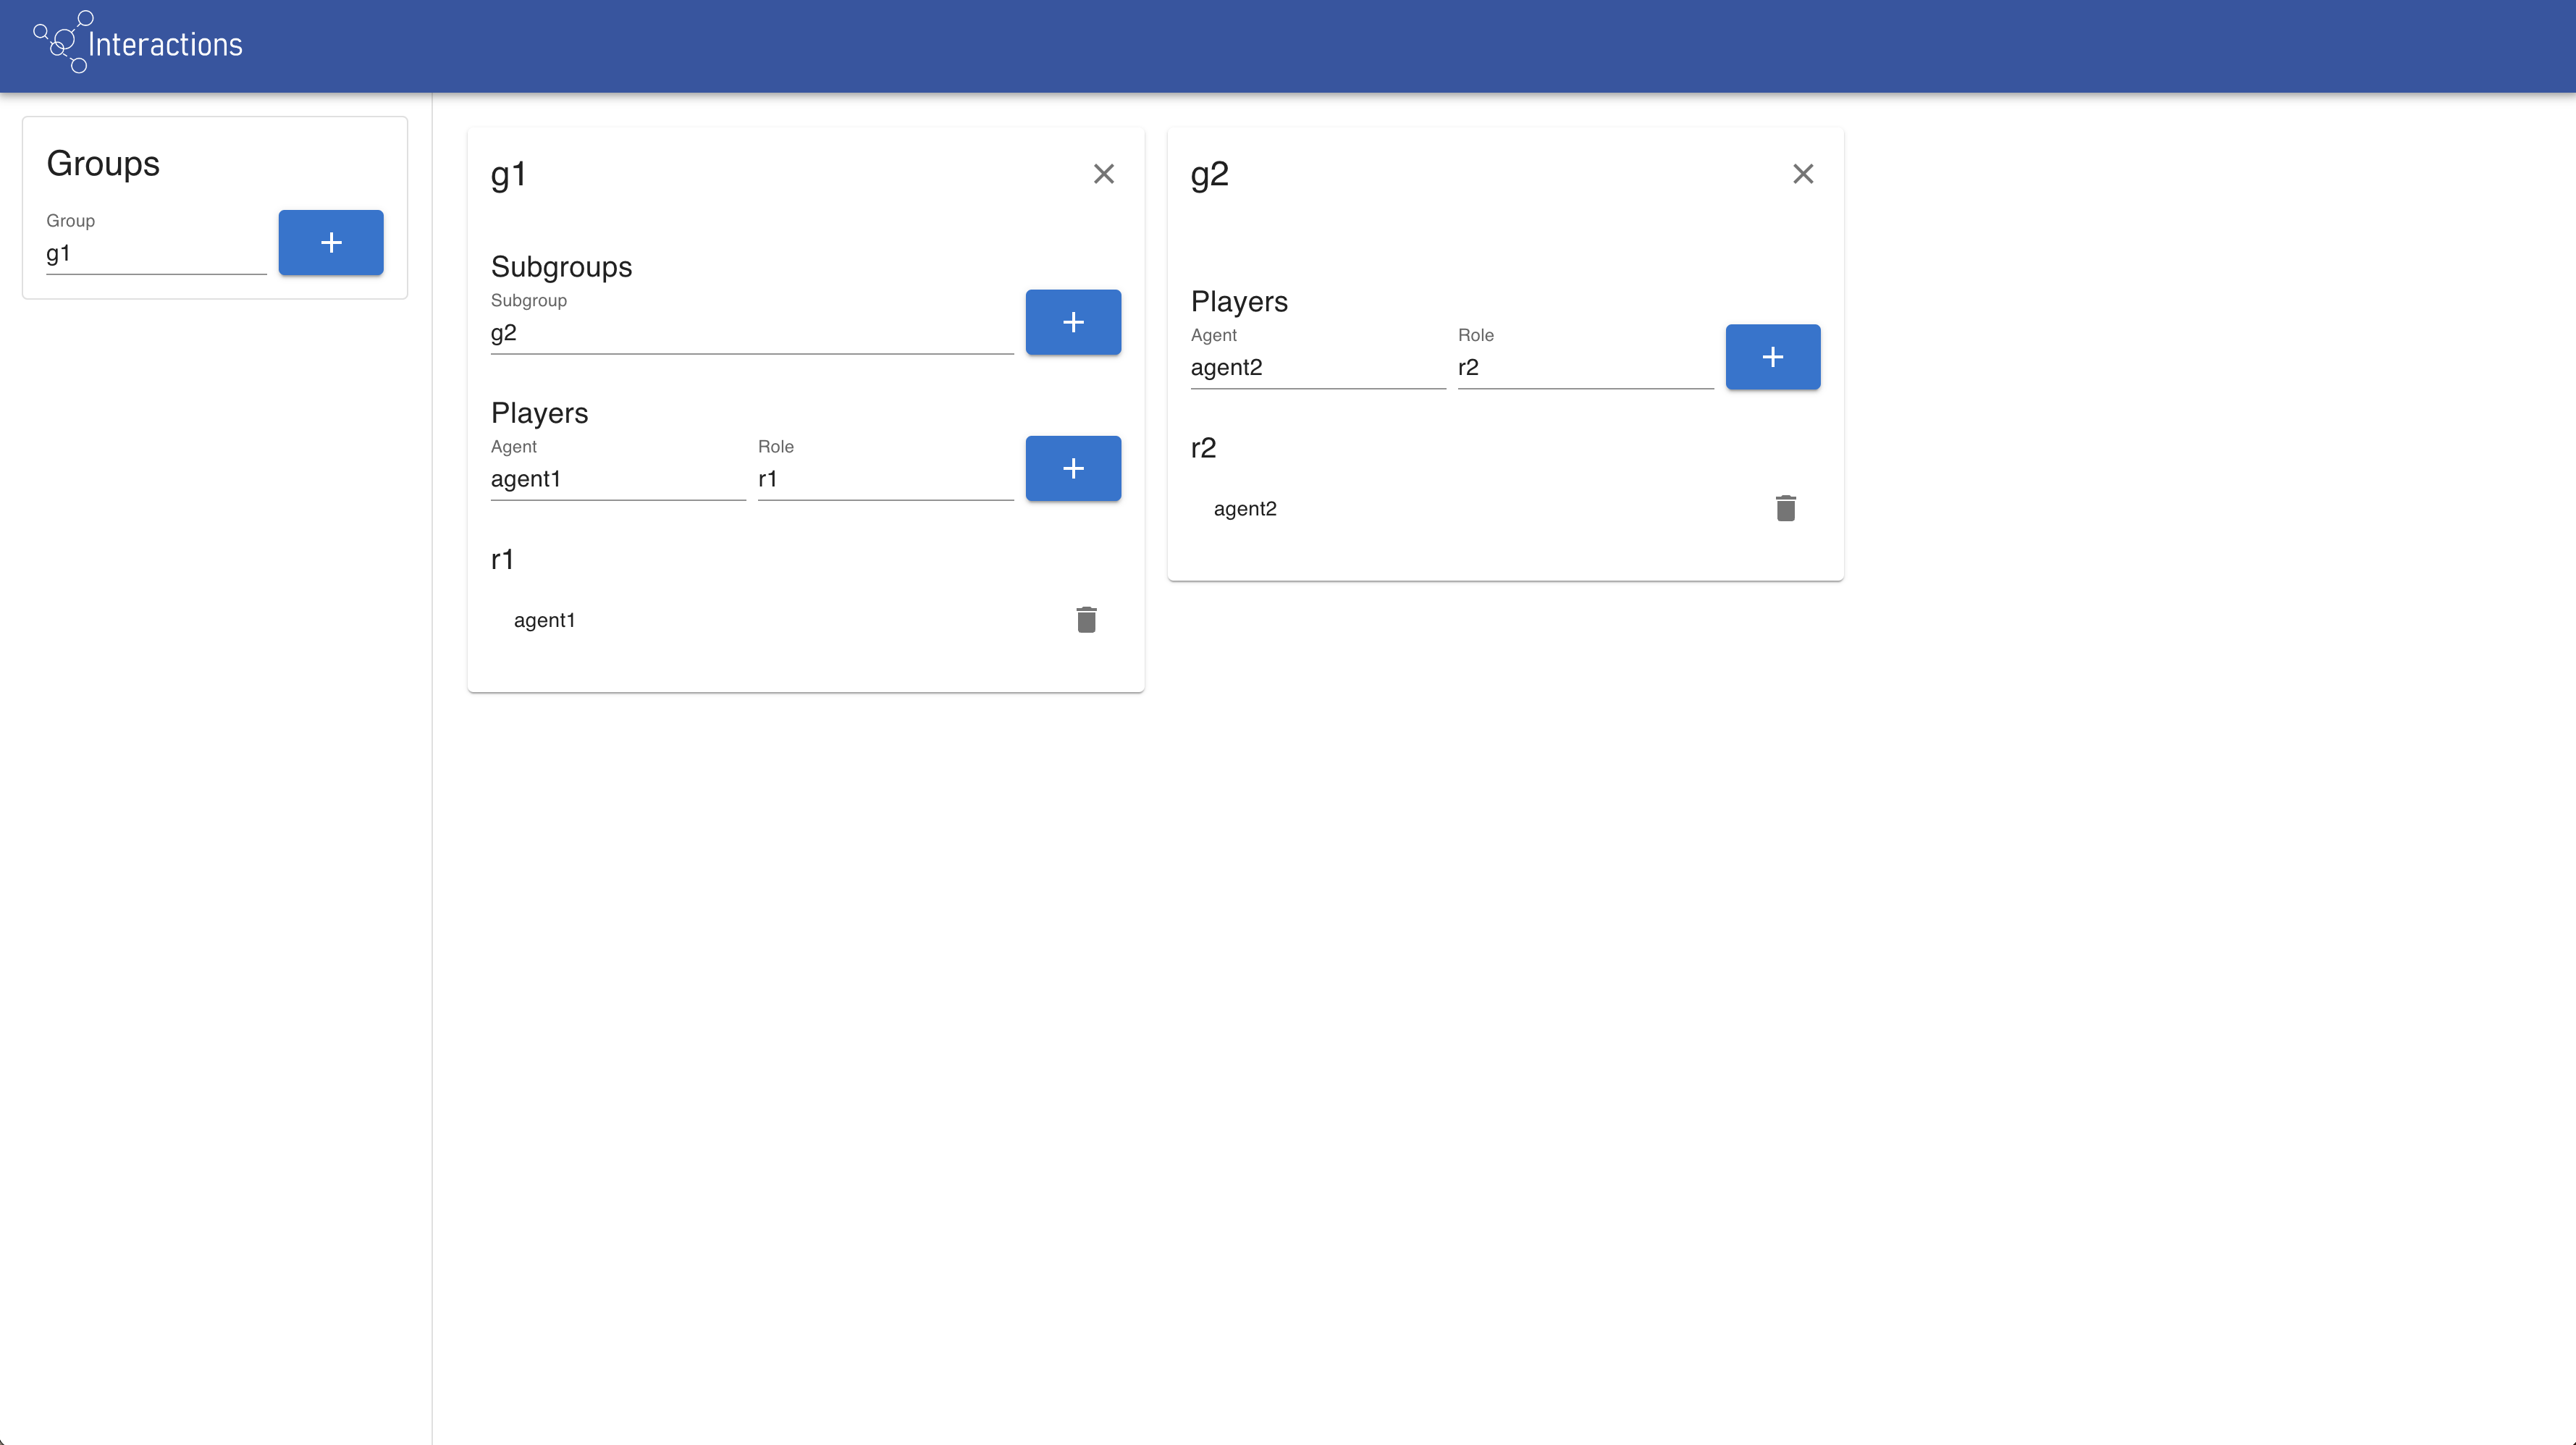
\includegraphics[width=\textwidth]{images/ide/entity.png}
    \end{figure}
\end{frame}

\subsection{Integration with the Runtime Environment}
\begin{frame}{Integration with the Runtime Environment}
    \begin{itemize}
        \item To deploy the created organizations, integration with the runtime environment is needed
        \item Domain experts can:
        \begin{itemize}
            \item Specify which groups will be deployed
            \item Access the agents running in the runtime environment
            \item Assign roles to agents
        \end{itemize}
        \item {Organizational artifacts}, which keep the information about the organization at runtime, are created
        \item Agents are told to join the organization and adopt the roles they were assigned
    \end{itemize}
\end{frame}
\section{Evaluation}

\begin{frame}[allowframebreaks]{Example}
    \begin{figure}
        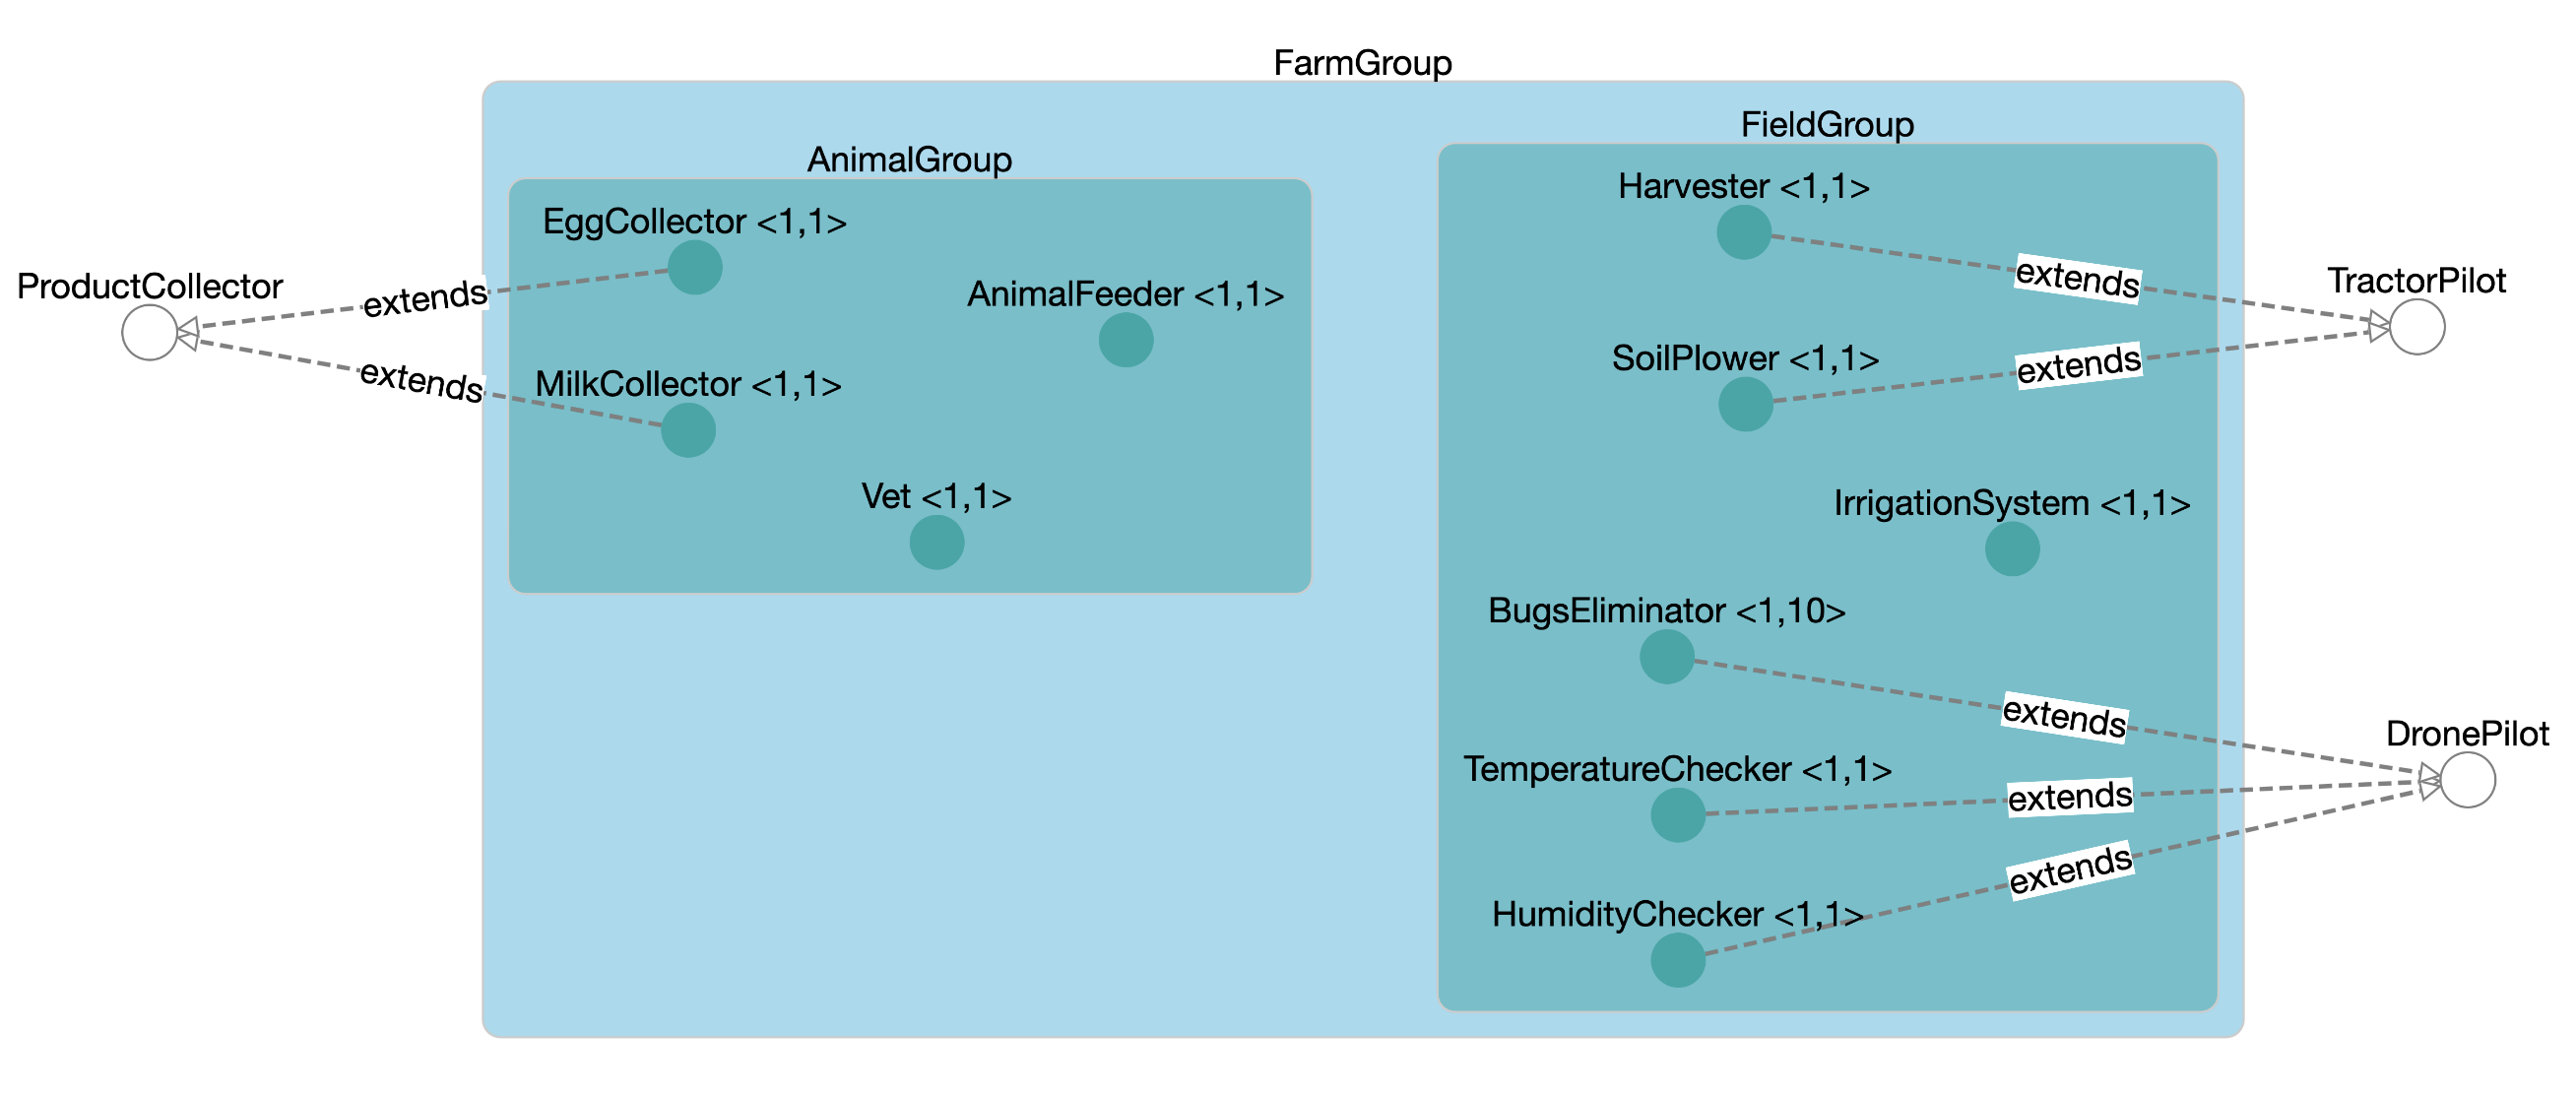
\includegraphics[width=\textwidth]{images/solution-structural.png}
    \end{figure}

    \framebreak

    \begin{figure}
        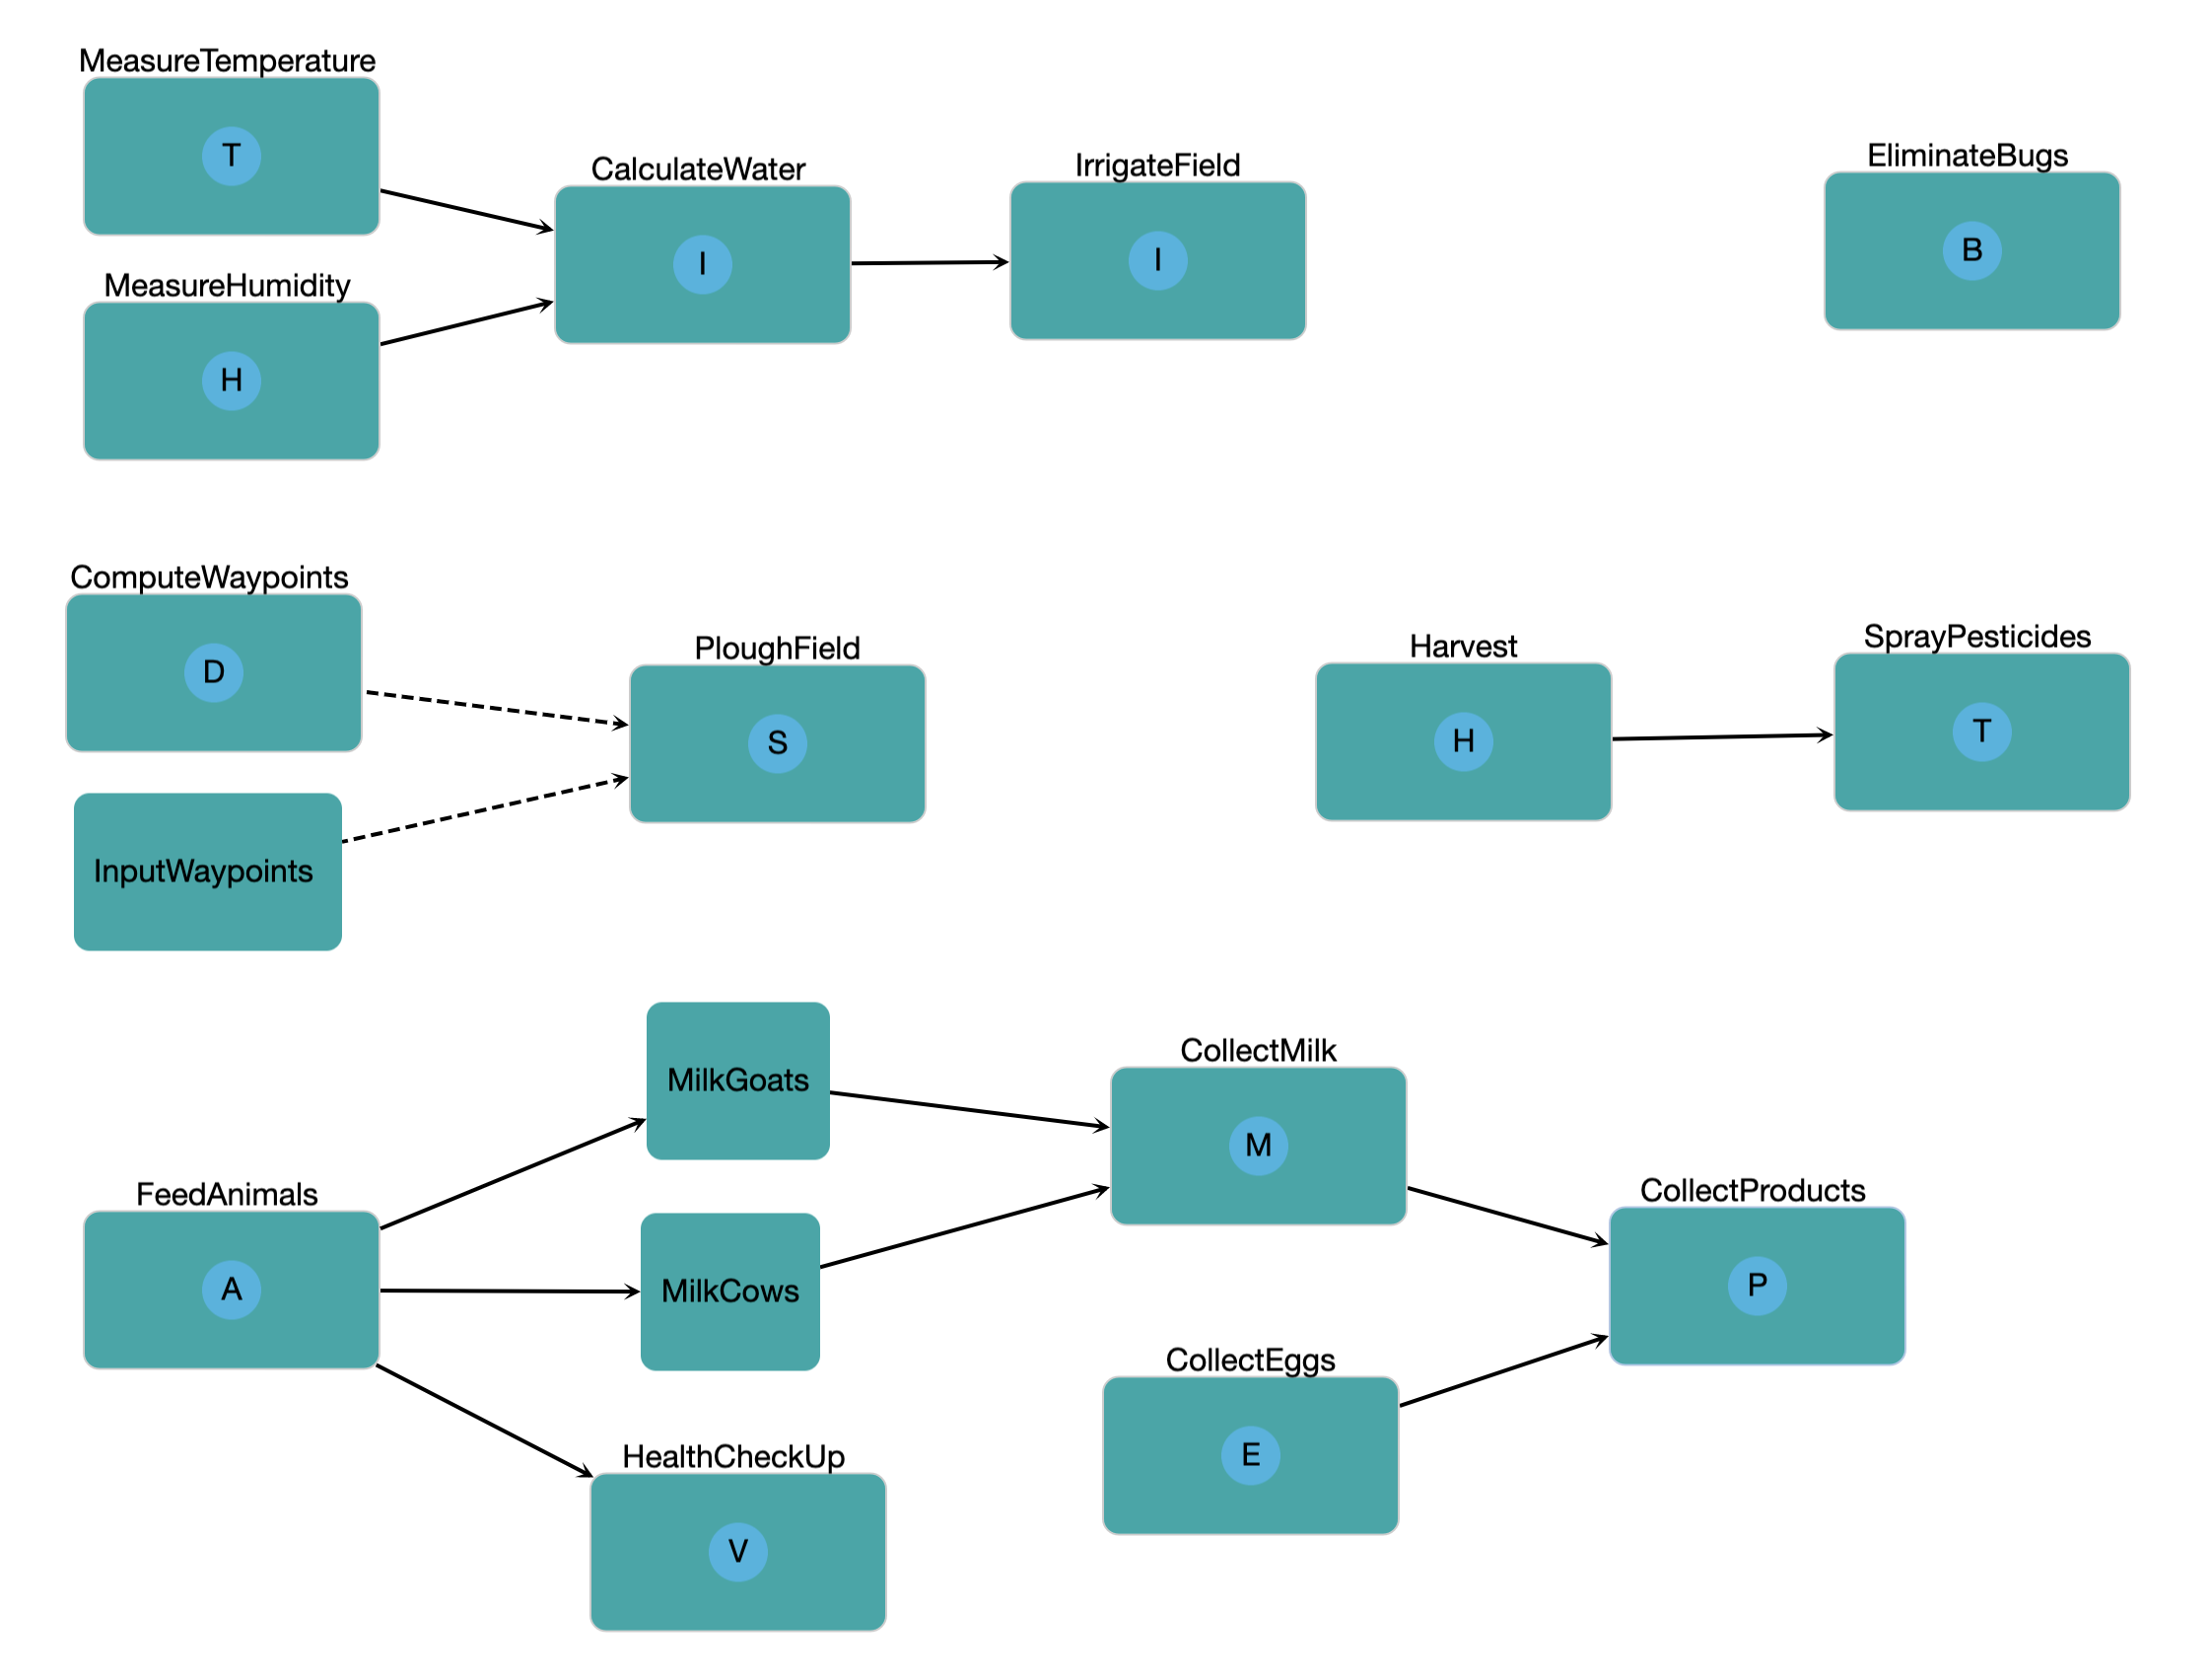
\includegraphics[width=0.8\textwidth]{images/solution-functional.png}
    \end{figure}
\end{frame}

\begin{frame}{Users' Test}
    

    \begin{columns}
        \begin{column}{0.4\textwidth}
            \begin{itemize}
                \item A test with end users was carried out to validate the prototype
                \item They were asked to perform tasks and rate the usability of the system
            \end{itemize}
        \end{column}
        \begin{column}{0.6\textwidth}
            \vspace{-0.5cm}
            \begin{figure}
                \centering
                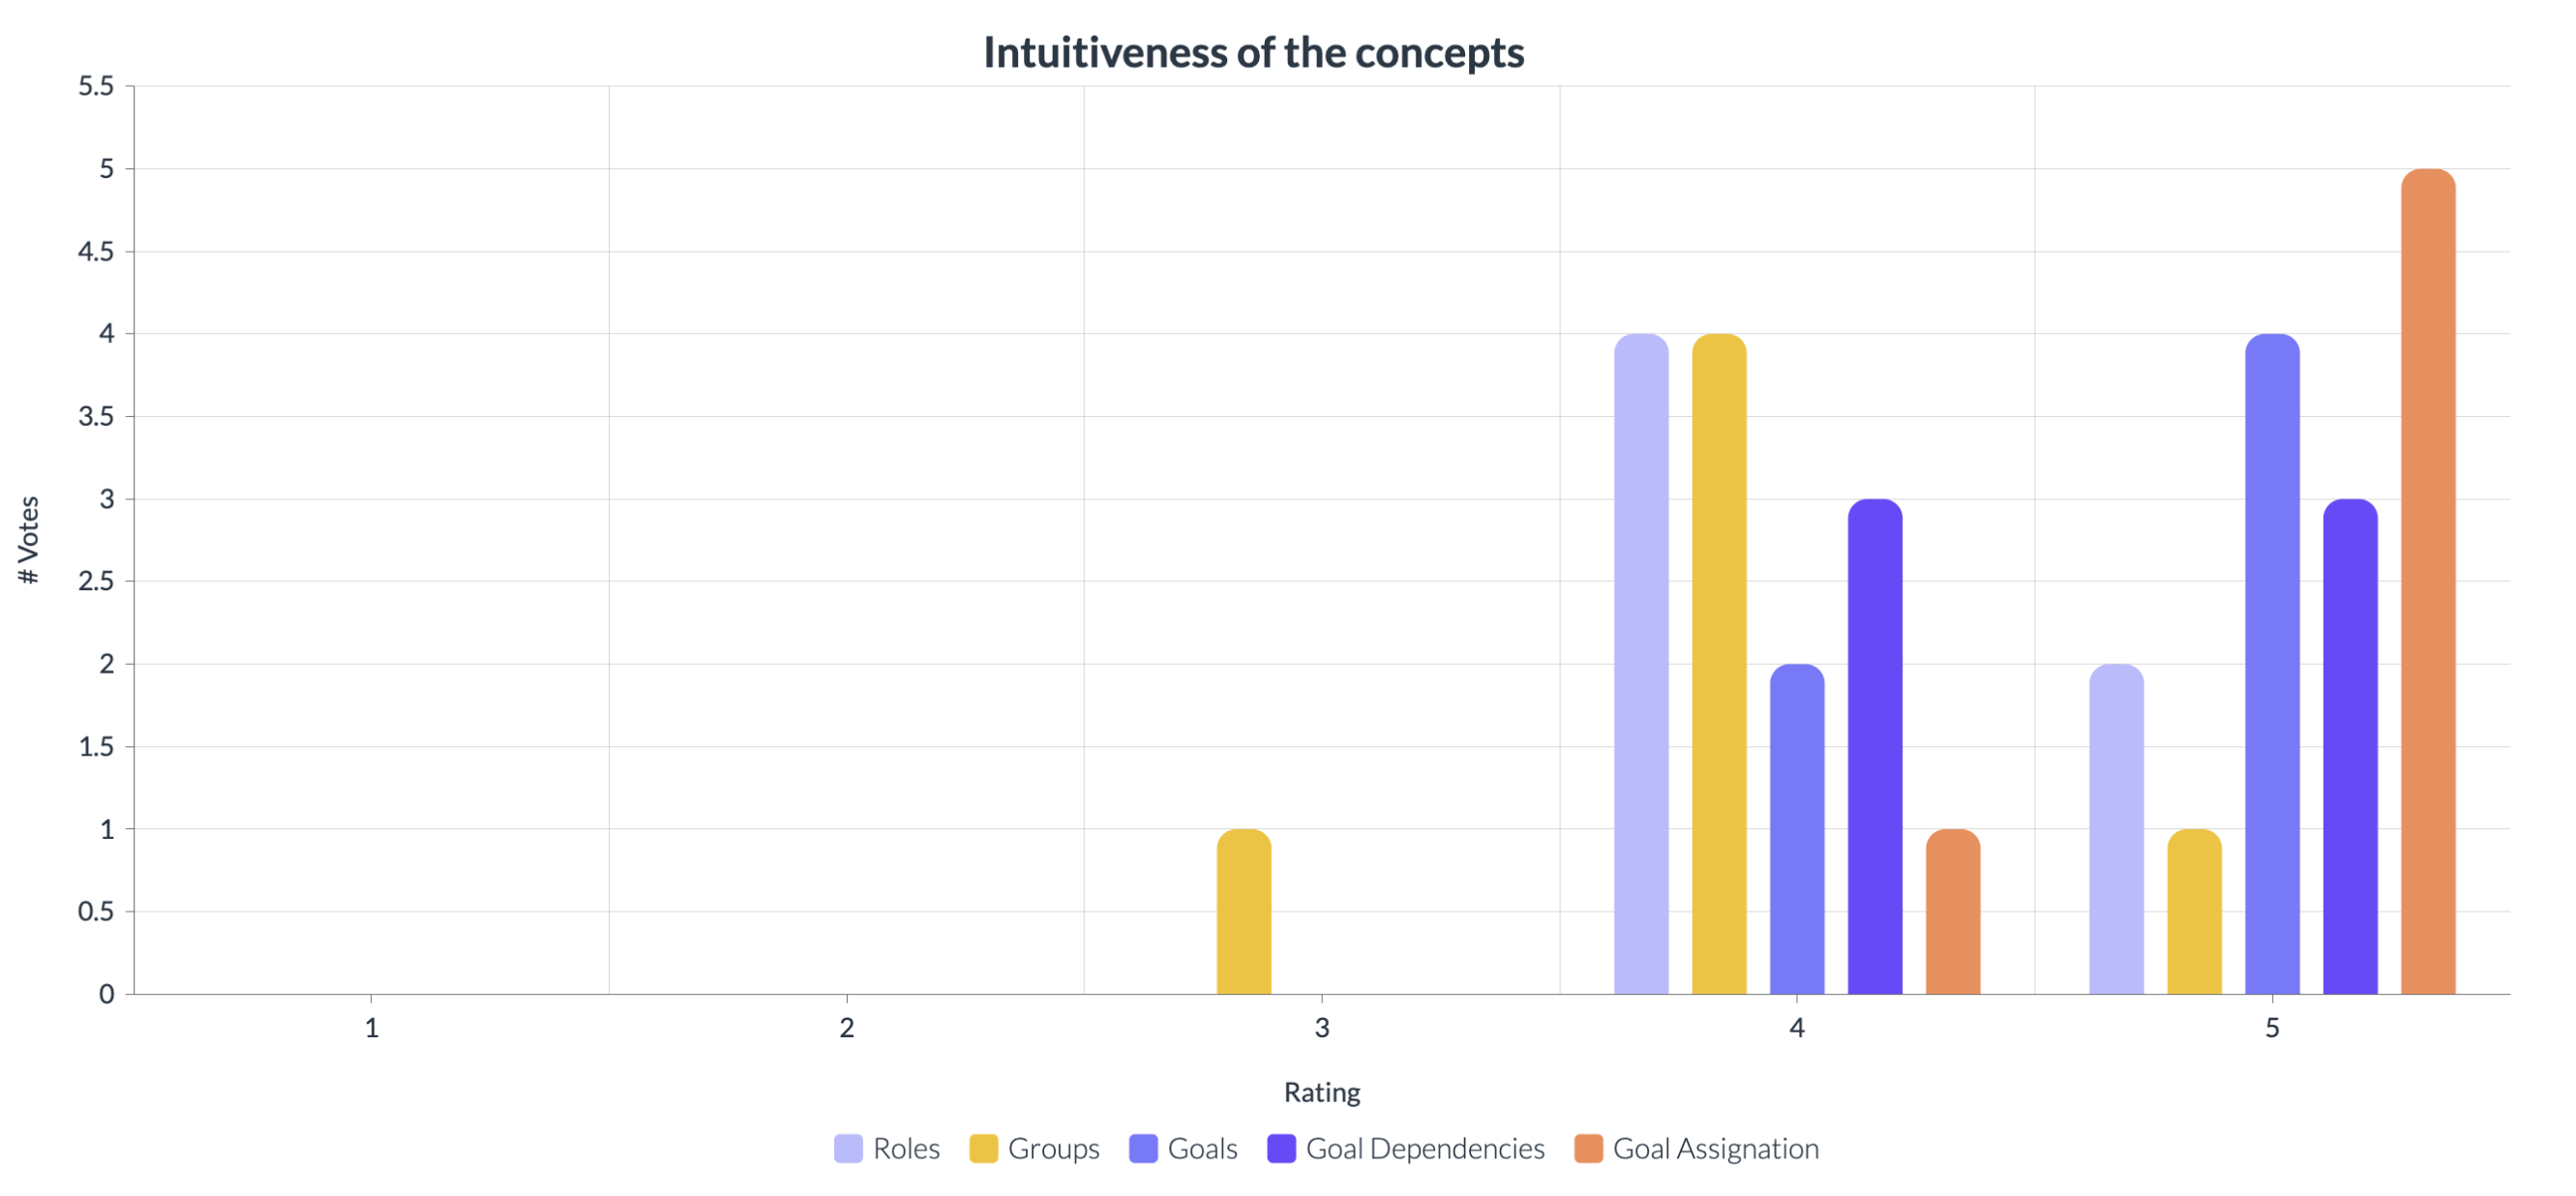
\includegraphics[width=\textwidth]{images/intuitiveness.png}
            \end{figure}
            \begin{figure}
                \centering
                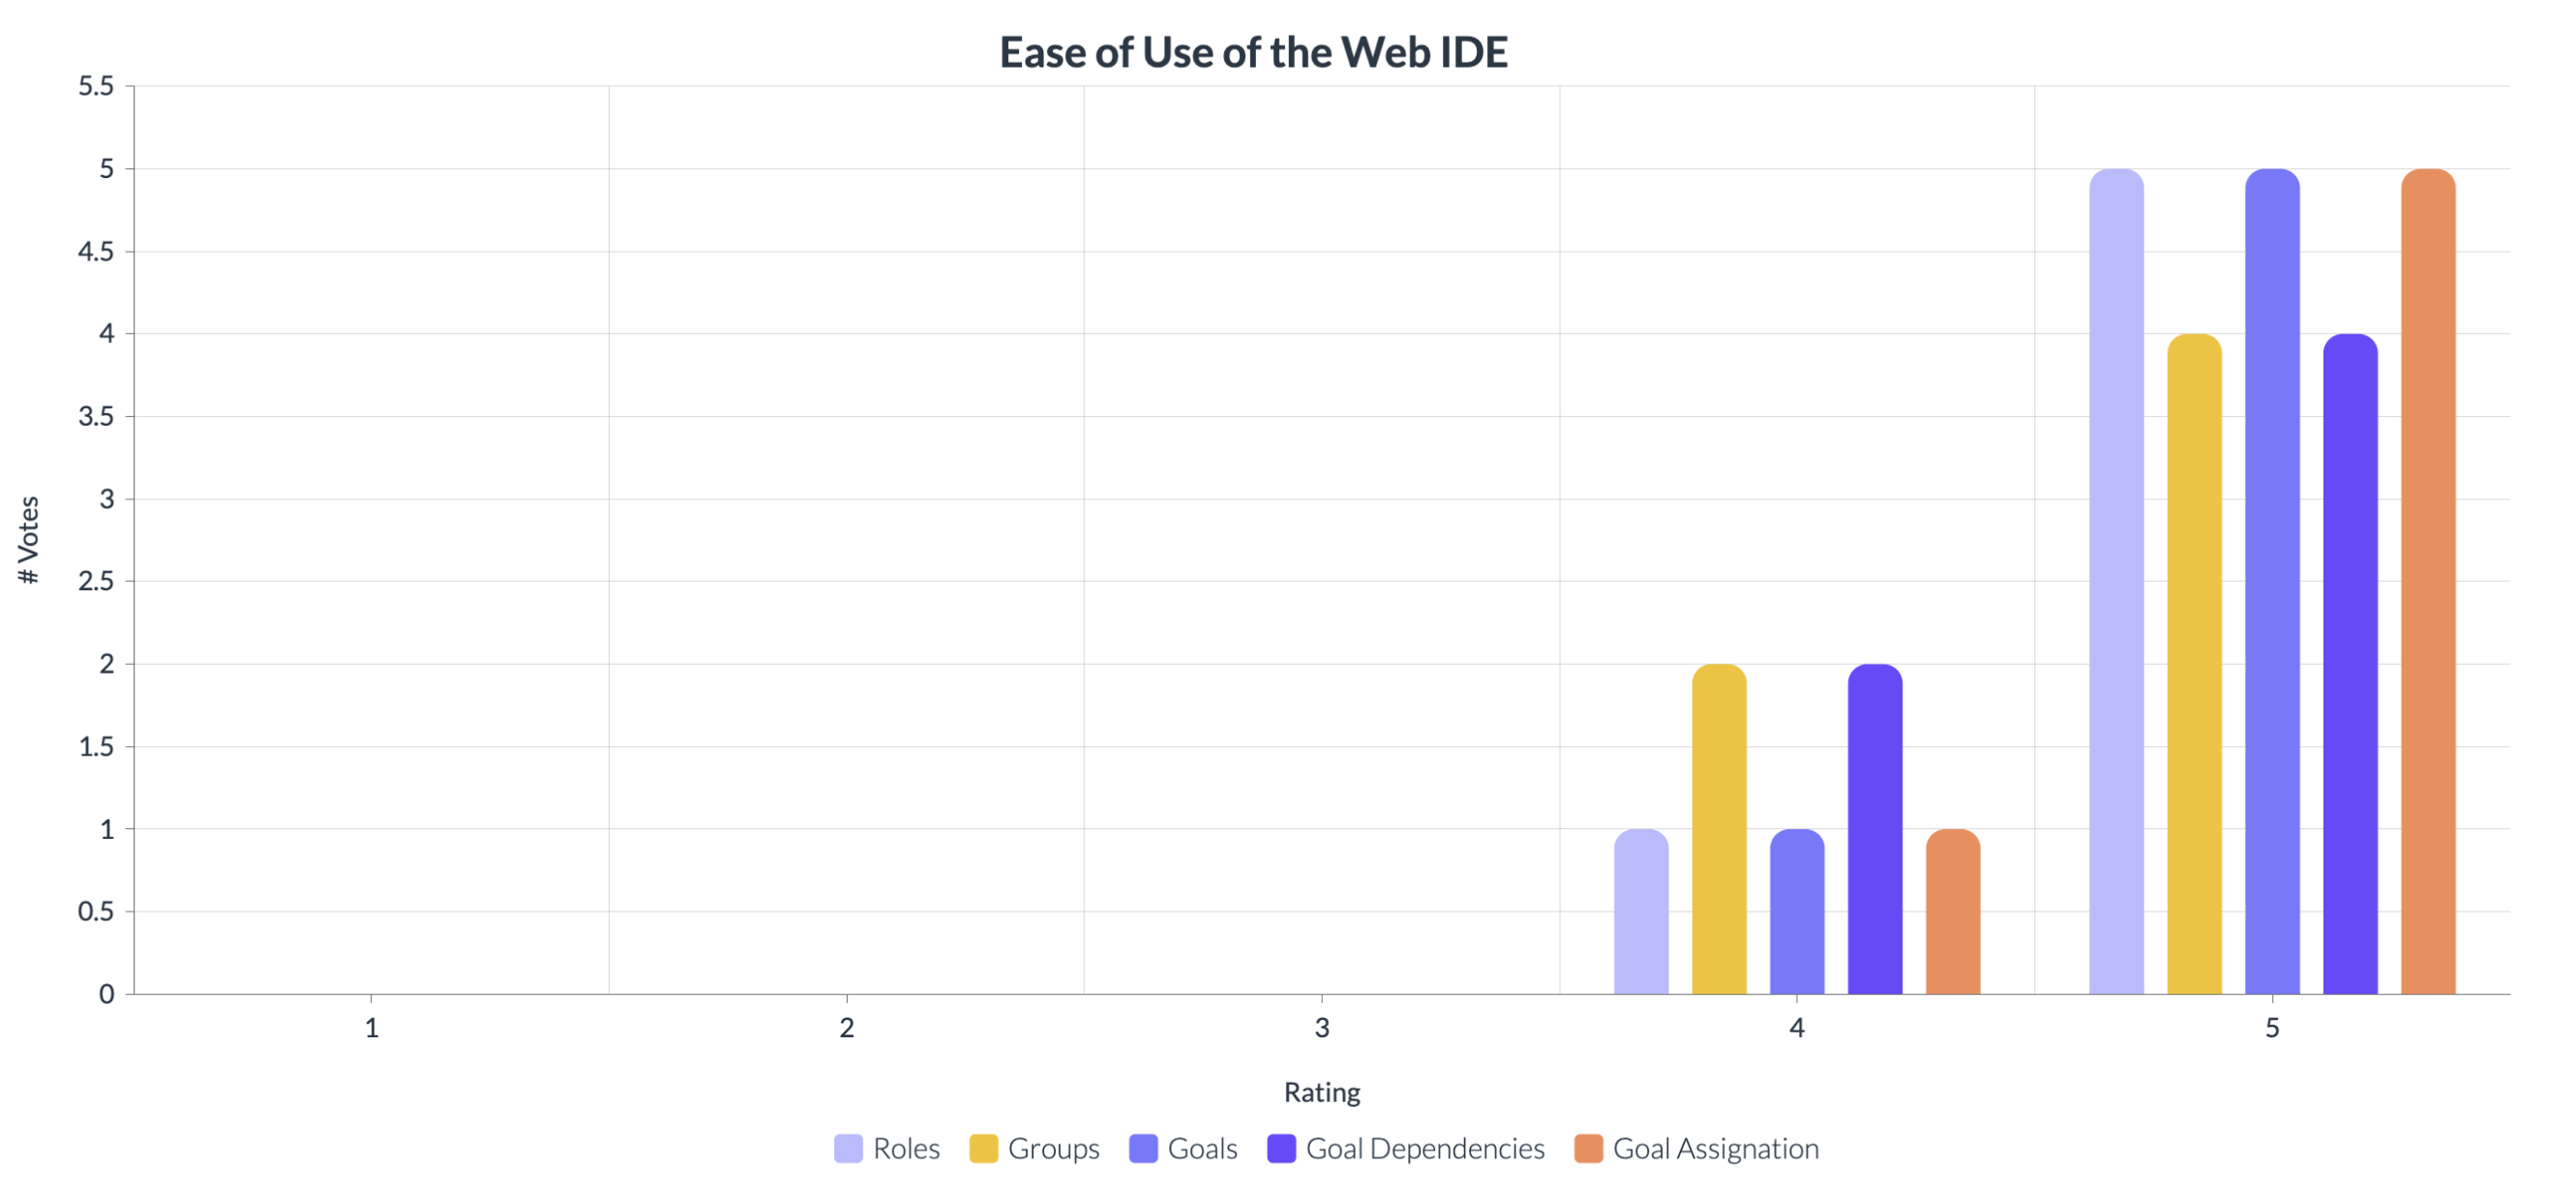
\includegraphics[width=\textwidth]{images/easeofuse.png}
            \end{figure}
        \end{column}
    \end{columns}
\end{frame}
\section{Conclusions}
\begin{frame}{Conclusions \& Future Work}
    \begin{itemize}
        \item The work culminated with the creation of a \textbf{Web IDE prototype} for the creation and \textbf{enforcement at runtime} of MAS organizations with a \textbf{visual language}
        \vspace{1cm}
        \item This project opens many possible directions for future works:
        \begin{itemize}
            \item Refinement of the visual language
            \item Exploration of other technologies
            \item Monitoring of the runtime state of the organizations
            \item Achievement of \emph{self-organization} and \emph{re-organization}
        \end{itemize}
    \end{itemize}
\end{frame}

\section*{}
\begin{frame}
    \titlepage
\end{frame}

\section*{\refname}
\setbeamertemplate{page number in head/foot}{}
\begin{frame}[t,allowframebreaks,noframenumbering]{References}
    \printbibliography
\end{frame}

\end{document}